\documentclass[conference]{IEEEtran}
\IEEEoverridecommandlockouts
\usepackage{cite}
\usepackage{amsmath,amssymb,amsfonts}
\usepackage{algorithmic}
\usepackage{graphicx}
\usepackage{dblfloatfix}
\usepackage{textcomp}
\usepackage{xcolor}
\usepackage{booktabs}
\usepackage{array}
\usepackage{url}

\graphicspath{{./}{figures/}}

% Float placement: loosen the defaults so figures settle near their
% references instead of piling up at the end of the document.
\renewcommand{\topfraction}{0.92}
\renewcommand{\bottomfraction}{0.85}
\renewcommand{\textfraction}{0.06}
\renewcommand{\floatpagefraction}{0.75}
\renewcommand{\dbltopfraction}{0.92}
\renewcommand{\dblfloatpagefraction}{0.75}
\setcounter{topnumber}{4}
\setcounter{bottomnumber}{3}
\setcounter{totalnumber}{6}
\setcounter{dbltopnumber}{3}

% \linebreakand: an \and that also starts a new, centered row of author
% blocks (useful when 5+ author blocks would otherwise leave a ragged last row).
\makeatletter
\newcommand{\linebreakand}{%
  \end{@IEEEauthorhalign}
  \hfill\mbox{}\par
  \mbox{}\hfill\begin{@IEEEauthorhalign}
}
\makeatother

\def\BibTeX{{\rm B\kern-.05em{\sc i\kern-.025em b}\kern-.08em
    T\kern-.1667em\lower.7ex\hbox{E}\kern-.125emX}}

\begin{document}

\title{Drift Detection and Reliability Analysis for Deployed ML Models}

% Emails below are placeholders in the institutional format;
% replace them with the real addresses before submission.
\author{%
\IEEEauthorblockN{Sanjay Mirchandani}
\IEEEauthorblockA{\textit{Department of Computer Engineering}\\
\textit{V.E.S. Institute of Technology}\\
Mumbai, India\\
sanjay.mirchandani@ves.ac.in}
\and
\IEEEauthorblockN{Nathan Cherian}
\IEEEauthorblockA{\textit{Department of Computer Engineering}\\
\textit{V.E.S. Institute of Technology}\\
Mumbai, India\\
2023.nathan.cherian@ves.ac.in}
\and
\IEEEauthorblockN{Rahul Guhagarkar}
\IEEEauthorblockA{\textit{Department of Computer Engineering}\\
\textit{V.E.S. Institute of Technology}\\
Mumbai, India\\
2023.rahul.guhagarkar@ves.ac.in}
\linebreakand
\IEEEauthorblockN{Alok Pal}
\IEEEauthorblockA{\textit{Department of Computer Engineering}\\
\textit{V.E.S. Institute of Technology}\\
Mumbai, India\\
2023.alok.pal@ves.ac.in}
\and
\IEEEauthorblockN{Akul Patre}
\IEEEauthorblockA{\textit{Department of Computer Engineering}\\
\textit{V.E.S. Institute of Technology}\\
Mumbai, India\\
2023.akul.patre@ves.ac.in}
}

\maketitle

\begin{abstract}
Machine learning models often lose accuracy after deployment. The data arriving in production drifts away from the training data. This usually happens before reliable labels are available. Existing monitoring tools signal that a distribution has changed. They say little about how much accuracy was lost, what caused it, which predictions to distrust or whether retraining will help. This paper presents a model agnostic monitoring pipeline that runs the full chain without production labels. It estimates performance, detects and locates drift, explains the likely cause, scores the reliability of each prediction and advises on remediation. Two parts are new. Image drift causes are reported as named visual concepts, for example a shift toward night photography. The ranking is checked against the image dataset's own tags. A remediation triage runs the two cheapest label free repairs as probes and predicts whether a full retrain will recover the loss. We evaluate on real drift and on injected drift. The real study uses the Folktables American Community Survey Income task and the Continual Learning on Real World Imagery benchmark. The injected study applies covariate, prior, concept and label noise shift with a known ground truth. The pipeline names the injected drift type in every tested window. The label free accuracy estimate is optimistic in every window. The model grows more confident as it grows less accurate. Per prediction reliability separates errors only under covariate shift. The concept level analysis agrees with the dataset tags at a rank correlation of $0.71$. The triage verdict matches whether any strategy recovers the loss across all tested settings.
\end{abstract}

\begin{IEEEkeywords}
data drift, concept drift, model monitoring, root cause analysis, out of distribution detection, model calibration, remediation, drift injection benchmark
\end{IEEEkeywords}

\section{Introduction}

A model that runs in production can quietly lose accuracy as the incoming data moves away from the training distribution. The loss usually begins long before reliable labels are available \cite{sculley2015hidden,paleyes2022challenges,huyen2022designing,shankar2022operationalizing}. Monitoring therefore has to catch the change and judge its effect while no labels are in hand.

Tools that already exist are good at announcing that a distribution has changed. They say much less about how much accuracy was lost, what caused the loss, which individual predictions should not be trusted or whether an expensive fix such as retraining is worth running \cite{klaise2020monitoring,rabanser2019failing}. A drift alert on its own is not an accuracy drop. An accuracy drop on its own is not a plan.

The pipeline proposed here treats monitoring as one workflow. The user supplies only a model and two sets of data: a reference set that stands for training and a stream of production data. The pipeline then estimates performance, detects and locates drift, explains the likely cause, scores the trust due to each prediction and advises on what to do. The same workflow serves a tabular model and an image model. Nothing in it needs production labels.

This paper makes four contributions.
\begin{enumerate}
\item An integrated label free workflow that connects performance estimation, drift detection, feature and slice level localization, root cause analysis, per prediction reliability scoring and remediation advice. Most existing tools stop at one of these steps.
\item Concept level visual root cause analysis. The pipeline turns drifted image embedding directions into ranked natural language concepts, for example a shift toward night photography. It checks the ranking against the image dataset's own tags.
\item A remediation triage. It runs the two cheapest label free repairs as probes and predicts whether a full retrain will recover the accuracy loss, before any retrain is run.
\item A controlled drift injection benchmark. It grades every stage of a label free monitor against a known ground truth, across covariate, prior, concept and label noise drift.
\end{enumerate}

The rest of the paper reviews related work, describes the architecture, gives the experimental setup for both the real and the injected studies, reports results and closes with a comparison, the limitations and future work.

\section{Related Work}
\label{sec:related_work}

Research on deployed model monitoring spans drift detection, representation learning, label free performance estimation, uncertainty, explanation and adaptation. The pipeline in this paper draws these threads into one flow. This section reviews each thread and states how the present work relates to it.

\subsection{Concept drift and dataset shift detection}
Surveys of concept drift cover detection and adaptation in changing data streams \cite{gama2014survey,lu2019learning,webb2016characterizing}. Distribution shift is usually split into covariate shift, prior shift and concept shift \cite{moreno2012unifying,quionero2009dataset}. Label based detectors such as Adaptive Windowing need labels to work \cite{bifet2007learning}, so label free methods compare the inputs or their learned features instead. Rabanser et al. show that the effectiveness of a detector depends on the type and size of the shift, which argues for an ensemble \cite{rabanser2019failing}. This pipeline combines feature level Kolmogorov--Smirnov and Population Stability Index tests with a multivariate kernel test so the members cover each other's blind spots.

\subsection{Monitoring high dimensional data through representations}
Representation learning maps raw inputs to compact features \cite{bengio2013representation}. Shift can then be tested in the learned space rather than in pixels \cite{rabanser2019failing}. This pipeline monitors 512 dimensional embeddings from a frozen ImageNet Residual Network with 18 layers \cite{he2016deep}, using a kernel test, reconstruction error and a distance between fitted Gaussians. Arranging the embeddings as a feature table lets image monitoring reuse the tabular detectors.

\subsection{Performance estimation without production labels}
Delayed or missing production labels have motivated methods that estimate accuracy from model outputs alone. Examples are thresholded confidence \cite{garg2022atc}, comparison of confidence distributions \cite{guillory2021predicting} and Confidence Based Performance Estimation \cite{kivimaki2025performance,nannyml2023cbpe}. This pipeline uses a Confidence Based Performance Estimation signal to gate alerts and reserves held out labels for checking. Because confidence and calibration themselves change under shift \cite{ovadia2019trust}, the estimate needs the reliability checks described next.

\subsection{Uncertainty and reliability under distribution shift}
Neural networks are often miscalibrated \cite{guo2017calibration}. Ovadia et al. show that many stay confident as their accuracy falls under shift \cite{ovadia2019trust}. Baseline out of distribution scores use the softmax output \cite{hendrycks2017baseline}, while anomaly methods such as Isolation Forest flag rare inputs \cite{liu2008isolation}. This pipeline does not equate confidence with correctness. It combines confidence, out of distribution risk, stability under perturbation, calibration risk and consistency of explanations into one risk score per prediction.

\subsection{Explanation and concept level interpretation}
Shapley Additive Explanations attribute a prediction to its features \cite{lundberg2017unified}. Gradient weighted Class Activation Mapping highlights the image regions a model relies on \cite{selvaraju2017gradcam}. Testing with Concept Activation Vectors measures how much a human named concept influences a class, using gradients and a trained probe \cite{kim2018tcav}. This pipeline compares reference and production explanation patterns for diagnosis. For images it adds a concept probe built on a Contrastive Language Image Pretraining model \cite{radford2021clip,ilharco2021openclip}, which needs no gradients and no training and reports the shift as ranked phrases.

\subsection{Covariate shift correction and remediation}
Weighting the training loss by the density ratio between production and reference is the classic correction for covariate shift \cite{shimodaira2000,sugiyama2007}. Isotonic regression recalibrates a model's scores on a small labelled sample \cite{zadrozny2002}. Most monitoring work stops at the alert and leaves the choice of repair to the team. This pipeline treats the repair as a decision. It runs cheap label free repairs as probes and reports whether a full retrain is likely to help.

\subsection{Integrated monitoring and evaluation with injected shift}
Shift detection \cite{rabanser2019failing}, performance estimation \cite{kivimaki2025performance} and uncertainty analysis \cite{ovadia2019trust} answer different questions. Few systems connect them. Evaluations also tend to use real drift, where the true cause and the true accuracy loss are unknown, so a stage can only be judged on whether it fires. This paper connects the stages into one workflow and adds a benchmark that injects drift with a known ground truth, so each stage can be graded on whether its answer is correct.

\section{System Architecture}
\label{sec:architecture}

This section follows the data through the pipeline. Fig.~\ref{fig:architecture} shows the seven stages, labelled A to G. Stages D, E and F sit inside one diagnosis block in the figure. The user supplies a model and two sets of data. The pipeline puts both sets into a shared form, checks for drift, locates it, studies the cause, scores the trust due to each prediction and then advises on what to do. Every stage after detection is optional. When a later stage fails, the failure is logged and the results that succeeded are kept. Everything produced is written to one JavaScript Object Notation (JSON) file and shown in an interactive dashboard. The subsections below follow the labels in the figure.

\begin{figure*}[!t]
    \centering
    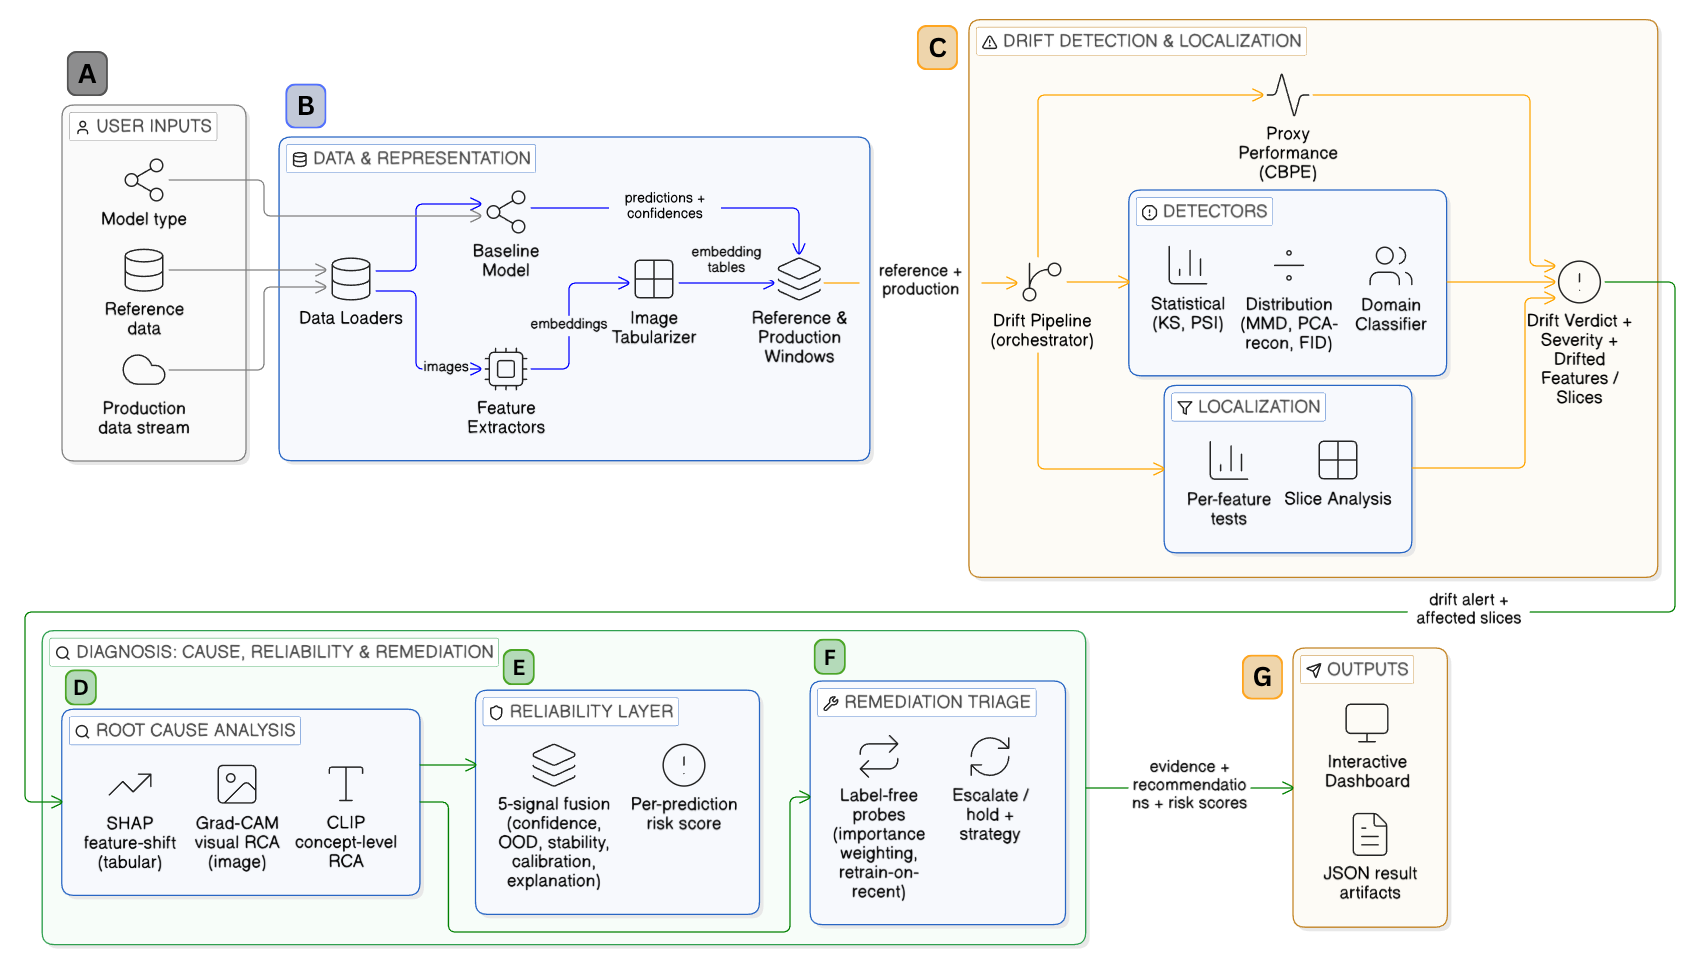
\includegraphics[
        width=0.94\textwidth,
        height=0.64\textheight,
        keepaspectratio
    ]{architecture.png}
    \caption{Data Drift Autopsy system architecture.}
    \label{fig:architecture}
\end{figure*}

\subsection{User input (A)}
The pipeline is built for a team that knows only two things: the type of model in production and the data it serves. The inputs are the trained model, a reference dataset that represents the training distribution and a stream of production data. Production labels are never required. The rest of the pipeline runs on these inputs alone.

\subsection{Data and representation (B)}
This stage gives tabular and image models one shared interface, so the same monitoring code serves both. Tabular inputs pass through schema validation, categorical encoding and treatment of missing values. Images are converted into 512 dimensional embeddings by an ImageNet pretrained Residual Network with 18 layers (ResNet-18) with its classification head removed \cite{he2016deep}. An image tabularizer then arranges these embeddings as a feature table with one column per dimension. This lets image drift reuse the tabular detectors without comparing raw pixels \cite{bengio2013representation,rabanser2019failing}. The baseline model produces predictions and class probabilities for the reference data and for each production batch. All of this is stored as reference and production windows. A window can use a fixed reference or the window that came just before it.

\subsection{Drift detection and localization (C)}
This stage asks whether the input distribution has moved and where the change sits. A pipeline orchestrator pairs one required detector with optional localization and cause analysis. The detector set is mixed on purpose. Table~\ref{tab:detectors} lists the members and the role of each.

\begin{table}[!htbp]
\caption{Drift detector ensemble.}
\label{tab:detectors}
\centering
\renewcommand{\arraystretch}{1.2}
\begin{tabular}{@{}p{1.9cm}p{2.1cm}p{3.0cm}@{}}
\toprule
\textbf{Detector} & \textbf{Statistic} & \textbf{Notes} \\
\midrule
KS test & Largest two sample KS statistic per feature; smallest $p$ & Numeric features; Bonferroni correction across features \\
PSI & Largest PSI per feature & Reference quantile bins; numeric and categorical features \\
MMD & Radial basis function kernel MMD; permutation $p$ & Multivariate; median bandwidth; 3000 row subsample \\
PCA reconstruction & Relative rise in reconstruction error & Embedding manifold; components retain 95\% variance \\
FID & Fr\'echet distance between fitted Gaussians & First and second moment shift in embeddings \\
CBPE & Chi-square statistic on confidence bins & Needs class probabilities; performance proxy \\
\bottomrule
\end{tabular}
\end{table}

Table~\ref{tab:detectors} gives the statistic behind each detector. The Kolmogorov--Smirnov (KS) test takes the largest per feature statistic and applies a Bonferroni correction \cite{massey1951kolmogorov}. The Population Stability Index (PSI) compares proportions across reference quantile bins through $(a-e)\ln(a/e)$ \cite{yurdakul2018statistical}. Maximum Mean Discrepancy (MMD) is a multivariate kernel test with a median bandwidth, permutation testing and a 3000 row subsample \cite{gretton2012kernel}. On image embeddings the pipeline also tracks the rise in Principal Component Analysis (PCA) reconstruction error and the Fr\'echet Inception Distance (FID) between fitted Gaussians \cite{heusel2017gans}.

A separate proxy stage estimates accuracy without labels. Reference and production top class confidences are placed in ten fixed bins. The bins are compared with Pearson's chi-square test, which is the Confidence Based Performance Estimation (CBPE) signal \cite{guillory2021predicting,kivimaki2025performance}. Accuracy is then estimated by reweighting the per bin accuracy of the reference with the production confidence histogram. Passing the chi-square $p$ value in place of the estimate is a category error, since the $p$ value is not a performance number. Labels are used only to check how good the estimate is.

Localization runs Bonferroni corrected KS tests on numeric features and chi-square tests on categorical features. It also compares data slices, which isolates census drift by state and image drift by class or by source. The stage ends with a drift verdict: a severity label, the list of drifted features and the affected slices. This verdict decides whether the later stages run.

\subsection{Root cause analysis (D)}
This stage links a detected shift to a change in how the model behaves. It does not prove cause. It narrows the search. For tabular models the pipeline computes mean absolute Shapley Additive Explanations (SHAP) attributions on 100 reference samples and 100 production samples \cite{lundberg2017unified}. The drifted features whose attribution has changed are the likely contributors. For image models the embedding dimensions that shifted are tied to the proxy estimate and to per class degradation. Gradient weighted Class Activation Mapping (Grad-CAM) overlays are drawn for the worst windows \cite{selvaraju2017gradcam}.

Grad-CAM shows where the model looks, not what changed in the data. To make the visual change readable the pipeline adds a concept probe. It uses a Contrastive Language Image Pretraining (CLIP) model \cite{radford2021clip,ilharco2021openclip} to compare each image against a fixed list of short phrases such as ``a night photo'' or ``a crowd of people''. For each image the phrase similarities are turned into a distribution with a softmax. Let $p_i(t_c)$ be the weight image $i$ places on phrase $c$. The concept mass shift is
\begin{equation}
\Delta_c = \frac{1}{n_{\mathrm{prod}}}\sum_{i} p_i^{\mathrm{prod}}(t_c) \;-\; \frac{1}{n_{\mathrm{ref}}}\sum_{i} p_i^{\mathrm{ref}}(t_c),
\label{eq:concept}
\end{equation}
where $n_{\mathrm{ref}}$ and $n_{\mathrm{prod}}$ are the reference and production sample sizes. A positive $\Delta_c$ means the production images lean more toward phrase $c$. The idea is related to concept activation testing \cite{kim2018tcav} but needs no gradients and no training. Section~\ref{sec:concept-results} checks the ranked phrases against dataset metadata.

\subsection{Reliability layer (E)}
Detection and cause analysis describe the population. This stage asks whether one particular prediction deserves trust. Each sampled prediction receives five scores in $[0,1]$. Confidence risk is one minus the top class probability. Out of distribution (OOD) risk comes from an Isolation Forest for tables \cite{liu2008isolation} and a percentile scaled distance for images \cite{hendrycks2017baseline}, both calibrated against the reference so that ordinary inputs score near zero. Instability is the mean change in the output under small input perturbations. Calibration risk is the gap between the confidence and the label free accuracy estimate. Explanation inconsistency is the change in the SHAP attribution pattern. The risk engine combines them as a weighted sum,
\begin{equation}
r = w_c(1-c) + w_o\,o + w_s\,s + w_k\,k + w_e\,e,
\label{eq:risk}
\end{equation}
where $c$, $o$, $s$, $k$ and $e$ are confidence, OOD risk, instability, calibration risk and explanation inconsistency. The default weights are $(0.20, 0.25, 0.20, 0.20, 0.15)$ and are renormalized when a signal is missing. A score below $0.33$ is low risk, up to $0.66$ is medium and above that is high. A few override rules catch clear cases, such as high confidence next to a high OOD score.

\subsection{Remediation triage (F)}
This stage turns the evidence into advice. A full retrain is expensive and does not always help, so the triage tests cheaper options first. It runs two label free repairs as probes. The first is importance weighted retraining on the reference data \cite{shimodaira2000,sugiyama2007}. Its weights come from a classifier trained to tell reference rows from production rows, whose predicted odds give the density ratio. The second is retraining on the most recent window. If a probe recovers at least one quarter of the estimated accuracy gap, the triage recommends escalating to a full retrain. If not, it reports that retraining is unlikely to help and points to collecting labels or checking the target rule. The pipeline also carries a wider set of strategies for offline study: feature dropping, a head refit and isotonic recalibration on a small labelled slice \cite{zadrozny2002}.

\subsection{Outputs (G)}
Every stage writes its result to one JSON file. This keeps partial runs useful and makes the analysis reproducible. An interactive dashboard reads the file. It presents the run as a step by step story for the two real datasets and as a controlled verification for the injected benchmark.

\section{Experimental Setup}

The pipeline is tested on one tabular task and one image task under real shifts. It is then tested on a benchmark of injected shifts with a known ground truth.

\subsection{Datasets}
The two real datasets stand for structured census records and for images ordered in time.

\textbf{American Community Survey (ACS) Income.} The Folktables income task uses ten demographic and employment features to predict whether income is above $\$50{,}000$ \cite{ding2021retiring}. California 2014 acts as the reference (183{,}941 rows; 35\% positive). California 2015 to 2018 give the temporal windows (187{,}475 to 195{,}665 rows). Texas, New York, Florida and Washington in 2014 give the geographic comparisons.

\textbf{Continual Learning on Real World Imagery (CLEAR).} The CLEAR-10 benchmark is ordered in time. It holds ten concepts plus a background class over ten buckets of roughly 3{,}300 images each \cite{lin2021clear}. Bucket 1 is the reference. Every later bucket is compared with the one before it.

\subsection{Models}
The models keep a linear decision rule so the two representations stay comparable. ACS uses standardized logistic regression trained on the 2014 reference, reaching an accuracy of $0.7985$. CLEAR-10 uses logistic regression on 512 dimensional ResNet-18 embeddings from a 70/30 reference split, reaching $0.849$ accuracy, $0.863$ macro precision, $0.849$ macro recall and a macro F1 score of $0.850$.

\subsection{Drift injection benchmark}
\label{sec:benchmark-setup}
Real drift has no ground truth, so a benchmark with injected drift is needed to grade the diagnosis. The reference is ACS Income for California in 2014. It is split into a training set of 20{,}000 rows, a reference set of 6{,}000 rows and a production pool of 4{,}800 rows. The model is the same standardized logistic regression. It reaches a reference accuracy of $0.7938$ on this smaller split, close to the full data value, with a positive rate of $0.35$. Four drift types are injected into copies of the production pool, each at three intensities, together with a no drift control. This gives 13 windows.

Covariate shift rescales the age and weekly hours features for a random half to two thirds of the rows, using $x' = \mu + s(x-\mu) + o\,\sigma$ with $s$ from $1.5$ to $3.2$ and $o$ from $0.8$ to $2.8$. The labels are left alone. Prior shift resamples whole rows so the positive rate moves from $0.35$ to $0.49$, $0.58$ or $0.67$. Each class keeps its feature profile. Concept drift inverts the label for the rows with the highest education value, covering the top $15$, $30$ or $50$ percent. No feature value is touched. Label noise flips a random $8$, $18$ or $32$ percent of labels with no feature dependence.

Each window is graded against its recipe. We record whether detection severity rises with intensity. We record the error of the label free accuracy estimate. We record the precision and recall of the localized features. We also record the area under the receiver operating characteristic curve (AUROC) of the reliability score against prediction error. A small delayed label audit of 600 labels is also run. It measures the accuracy drop and checks whether the loss sits in one feature range. A simple rule then reads these signals and names the drift type.

\subsection{Configuration and metrics}
Thresholds and sampling rules were fixed before any evaluation began. KS and CBPE alert at $p<0.05$. PSI alerts at $0.2$ for tables or $0.025$ for embeddings, MMD at $0.1$ or $0.02$, the rise in PCA reconstruction at $0.28$ and FID at $14.0$. Reliability sampling draws 200 tabular predictions and 80 image predictions per window, with fixed seeds and bin accuracy calibrated on the reference.

The evaluation reports how far detectors agree, the mean absolute error of the proxy against labels held back only for checking, agreement on which features were localized and the spread of reliability scores. Everything ran on a single workstation, where the graphics processing unit (GPU) was used only to build embeddings. The software stack was scikit-learn \cite{pedregosa2011scikit}, SciPy \cite{virtanen2020scipy}, NumPy \cite{harris2020array}, SHAP, OpenCLIP and PyTorch.

\section{Results and Discussion}

The results cover detection, localization, cause analysis, performance estimation, reliability, remediation and the injection benchmark, in the order the pipeline produces them.

\subsection{Temporal drift on ACS Income}
The first question is whether the monitoring signals move together with measured accuracy. Table~\ref{tab:acs-temporal} collects the yearly results.

\begin{table}[!htbp]
\caption{ACS Income temporal drift.}
\label{tab:acs-temporal}
\centering
\renewcommand{\arraystretch}{1.18}
\begin{tabular}{@{}lcccc@{}}
\toprule
\textbf{Window} & \textbf{2015} & \textbf{2016} & \textbf{2017} & \textbf{2018} \\
\midrule
Measured accuracy & 0.7925 & 0.7894 & 0.7846 & 0.7789 \\
Drop relative to 2014 & $-0.0059$ & $-0.0091$ & $-0.0139$ & $-0.0196$ \\
Estimated accuracy & 0.7982 & 0.7970 & 0.7945 & 0.7945 \\
\midrule
KS statistic & 0.0077 & 0.0160 & 0.0230 & 0.0369 \\
KS verdict & critical & critical & critical & critical \\
PSI & 0.0005 & 0.0013 & 0.0037 & 0.0342 \\
PSI verdict & none & none & none & none \\
MMD & 0.000 & 0.0099 & 0.000 & 0.0276 \\
MMD verdict & none & none & none & none \\
CBPE $\chi^2$ & 11.2 & 24.1 & 213.0 & 201.3 \\
CBPE verdict & medium & critical & critical & critical \\
\midrule
Mean confidence & 0.793 & 0.794 & 0.797 & 0.804 \\
Drifted features & 4 & 8 & 8 & 8 \\
\bottomrule
\end{tabular}
\end{table}

Table~\ref{tab:acs-temporal} gives the aggregate detector statistics, with CBPE shown through its chi-square value. Every KS and CBPE outcome stays significant after correction. Measured accuracy slides from $0.7925$ in 2015 to $0.7789$ in 2018, a $1.96$ point fall from the 2014 baseline. The corrected KS test calls the drift critical in every window and grows larger as accuracy shrinks. PSI and MMD stay under their thresholds, which says that the marginal changes are small even though the combined input shift can still be detected. CBPE goes from medium severity in 2015 to critical severity in every year after that, which shows that the confidence distribution of the model moves with the data. Fig.~\ref{fig:acs-detectors} draws these detector responses.

\begin{figure*}[!t]
    \centering
    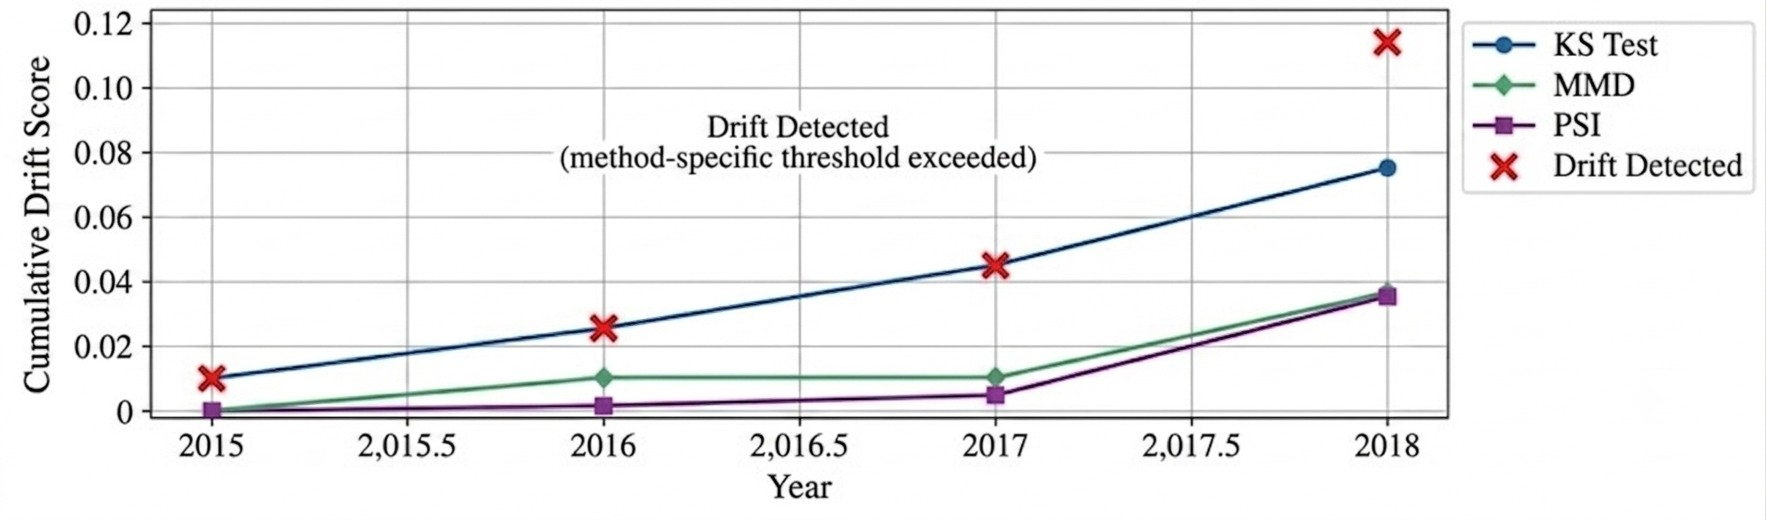
\includegraphics[width=0.90\textwidth]{7f3905fe-5a8e-4103-abfd-06179f7b2fe51.jpg}

    \vspace{1mm}
    (a)

    \vspace{2mm}

    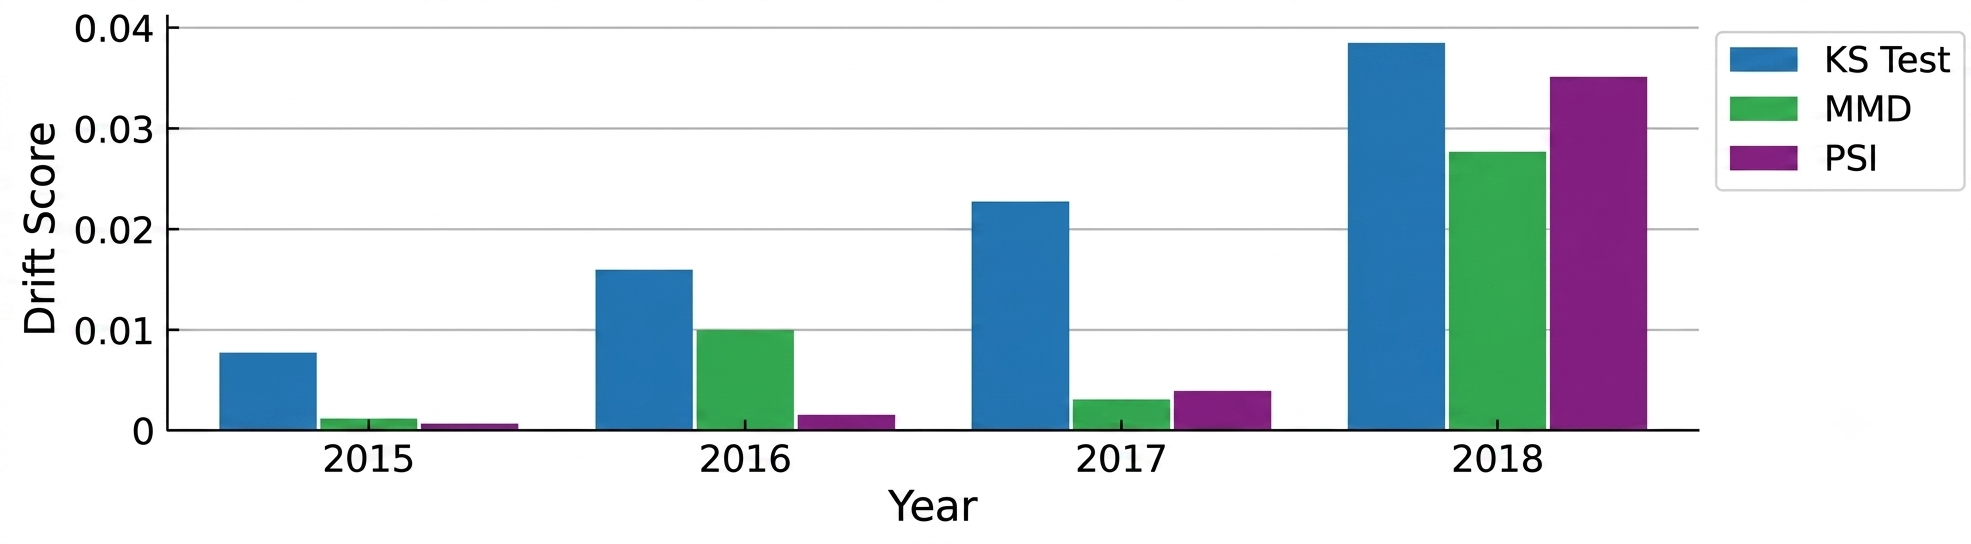
\includegraphics[width=0.90\textwidth]{7f3905fe-5a8e-4103-abfd-06179f7b2fe5.jpg}

    \vspace{1mm}
    (b)

    \caption{ACS Income detector trends: (a) cumulative detector scores with alert markers; (b) annual detector score comparison.}
    \label{fig:acs-detectors}
\end{figure*}

Panel (a) tracks the running detector score with a marker at each alert. Panel (b) compares the annual scores. The KS and CBPE curves climb every year while PSI and MMD stay near the axis, which is the same split seen in Table~\ref{tab:acs-temporal}.

A second pattern shows up in the confidence numbers. Accuracy drops by almost two points, yet mean confidence climbs from $0.793$ to $0.804$ and the CBPE mean shift stays positive in every window. The same growth in overconfidence under shift has been reported for deep networks \cite{ovadia2019trust,guo2017calibration}. The label free estimate sits $0.6$ to $1.6$ points above measured accuracy, because the confidence to accuracy mapping fitted on 2014 slowly goes stale. Fig.~\ref{fig:acs-confacc} sets the accuracy decline against the spread of detector severity.

\begin{figure*}[!t]
    \centering
    \begin{minipage}{0.45\textwidth}
        \centering
        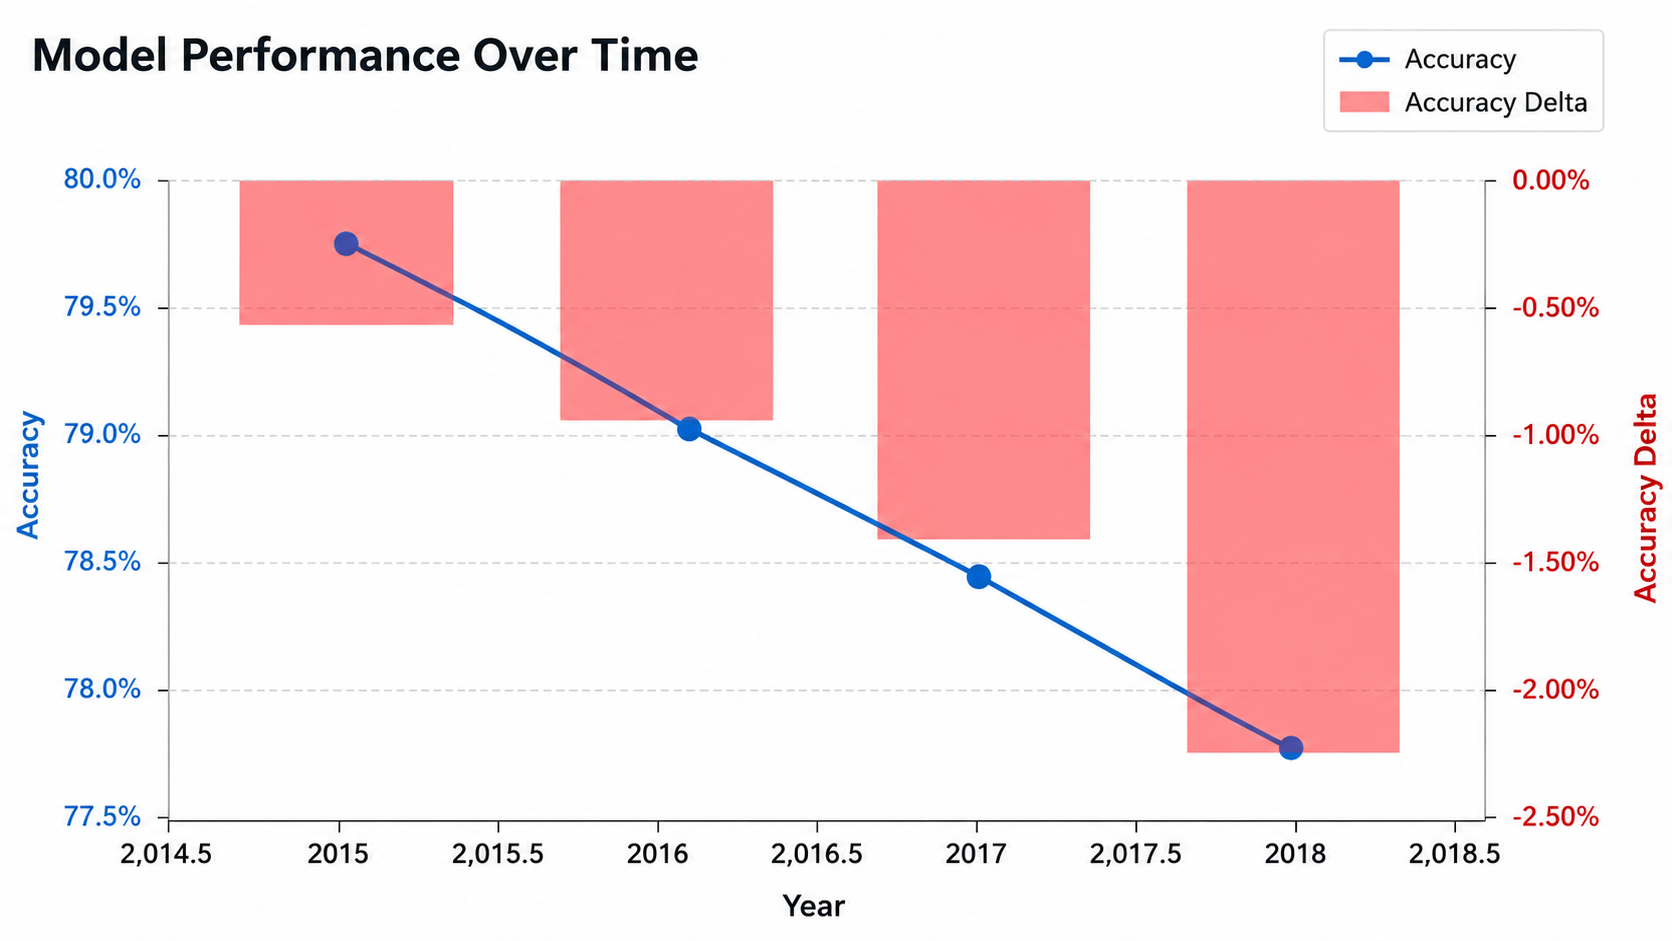
\includegraphics[width=\textwidth]{pinkgraph fixed.png}

        \vspace{1mm}
        (a)
    \end{minipage}
    \hfill
    \begin{minipage}{0.45\textwidth}
        \centering
        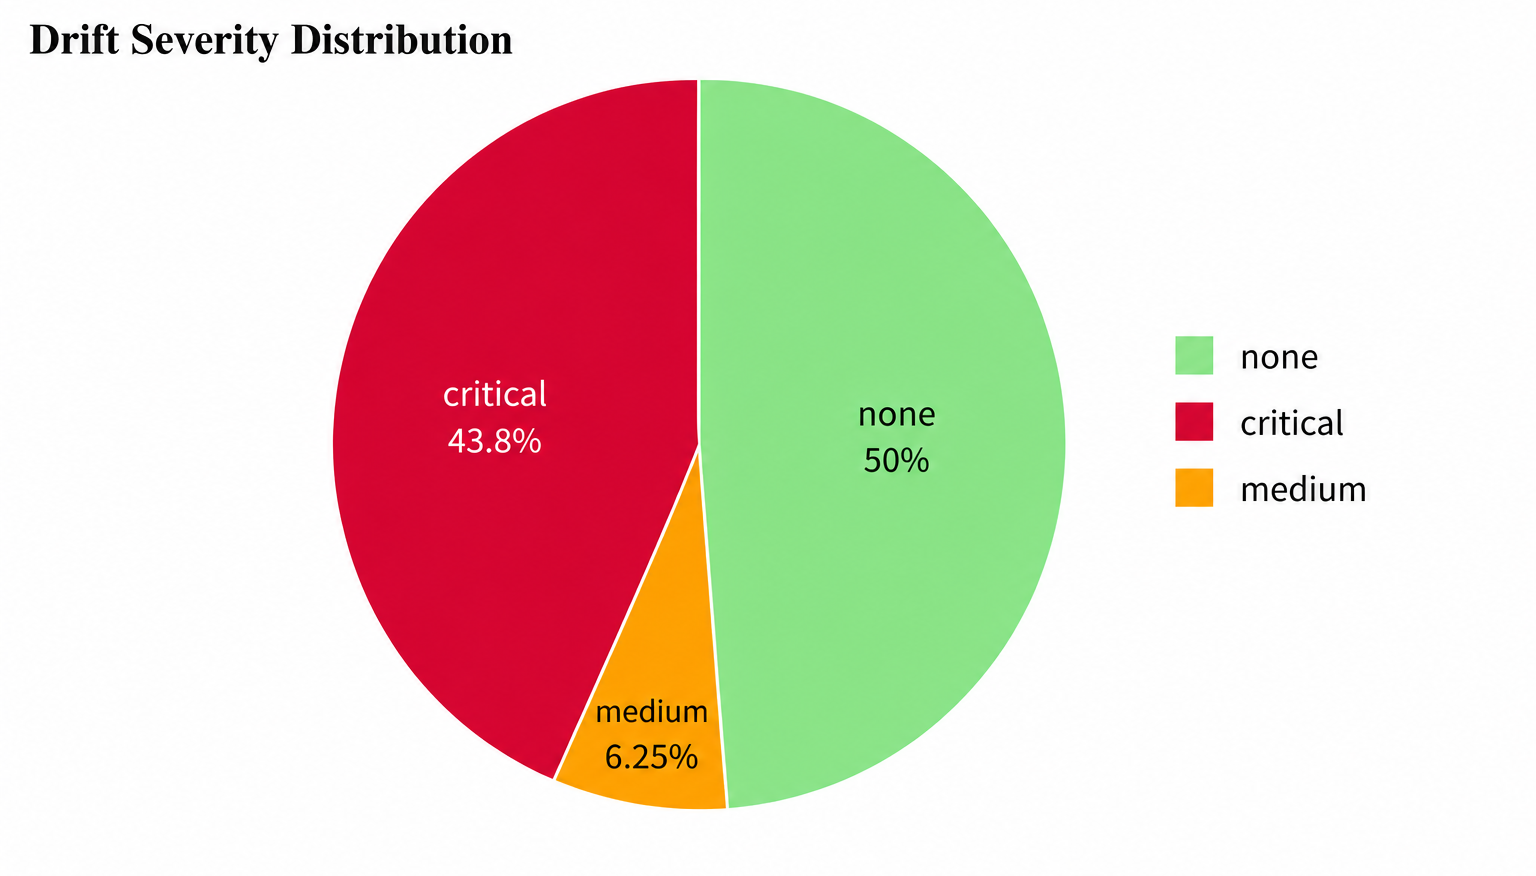
\includegraphics[width=\textwidth]{piechartfixed.png}

        \vspace{1mm}
        (b)
    \end{minipage}

    \caption{ACS Income performance summary: (a) measured accuracy with the change from the 2014 baseline; (b) distribution of drift severity.}
    \label{fig:acs-confacc}
\end{figure*}

Panel (a) plots measured accuracy with the year on year change. Panel (b) shows that almost every window lands at critical severity, driven by the KS and CBPE alerts rather than the multivariate tests.

The next step traces the yearly alerts down to single census variables. Table~\ref{tab:acs-features} uses the dataset codes for marital status (MAR), relationship (RELP), age (AGEP), educational attainment (SCHL), race (RAC1P), occupation (OCCP), place of birth (POBP) and weekly hours worked (WKHP).

\begin{table}[!htbp]
\caption{Localized ACS Income features.}
\label{tab:acs-features}
\centering
\renewcommand{\arraystretch}{1.2}
\begin{tabular}{@{}clp{4.6cm}@{}}
\toprule
\textbf{Window} & \textbf{Count} & \textbf{Drifted features} \\
\midrule
2015 & 4 & MAR, RELP, AGEP, SCHL \\
2016 & 8 & AGEP, SCHL, MAR, RELP, RAC1P, OCCP, POBP, WKHP \\
2017 & 8 & AGEP, SCHL, MAR, RELP, RAC1P, OCCP, POBP, WKHP \\
2018 & 8 & AGEP, SCHL, MAR, RELP, RAC1P, OCCP, POBP, WKHP \\
\midrule
\multicolumn{2}{@{}l}{Persistent} & AGEP, SCHL, MAR, RELP \\
\bottomrule
\end{tabular}
\end{table}

Table~\ref{tab:acs-features} shows four drifting features in 2015 and eight from 2016 onward. AGEP, SCHL, MAR and RELP drift in every window, so they stand for lasting change rather than a one off event. OCCP and POBP also change how the model behaves, which is the reason for the attribution study in Table~\ref{tab:acs-shap}.

\begin{table}[!htbp]
\caption{ACS Income attribution changes.}
\label{tab:acs-shap}
\centering
\renewcommand{\arraystretch}{1.2}
\begin{tabular}{@{}cll@{}}
\toprule
\textbf{Window} & \textbf{Reliance up} & \textbf{Reliance down} \\
\midrule
2015 & AGEP, SCHL, MAR & none \\
2016 & none & OCCP, POBP, AGEP \\
2017 & WKHP, AGEP, SCHL & OCCP, POBP \\
2018 & OCCP, POBP, SCHL & WKHP, AGEP, RELP \\
\bottomrule
\end{tabular}
\end{table}

Table~\ref{tab:acs-shap} keeps the SHAP comparison to drifted features only. Reliance on OCCP and POBP falls through 2016 and 2017 before rising again in 2018. From 2017 onward the likely root cause set settles around WKHP, SCHL, AGEP, POBP and OCCP. This sends an investigation toward the way occupation and place of birth were coded between survey years.

\subsection{Geographic drift on ACS Income}
The geographic study separates variation across places from the changes over time. California (CA) in 2014 stays as the reference. New York (NY), Florida (FL), Texas (TX) and Washington (WA) act as the production slices in Table~\ref{tab:acs-geo}.

\begin{table}[!htbp]
\caption{ACS Income geographic drift.}
\label{tab:acs-geo}
\centering
\renewcommand{\arraystretch}{1.2}
\begin{tabular}{@{}lcccc@{}}
\toprule
\textbf{Comparison} & \textbf{POBP} & \textbf{RAC1P} & \textbf{Drift count} & \textbf{CBPE $\chi^2$} \\
\midrule
CA $\rightarrow$ CA & 0.00 & 0.00 & 0 & $\approx 0$ \\
CA $\rightarrow$ NY & 0.487 & 0.161 & 10 & 1154 \\
CA $\rightarrow$ FL & 0.440 & 0.246 & 10 & 1795 \\
CA $\rightarrow$ TX & 0.423 & 0.198 & 9 & 543 \\
CA $\rightarrow$ WA & 0.350 & 0.173 & 9 & 577 \\
\bottomrule
\end{tabular}
\end{table}

Table~\ref{tab:acs-geo} lists the KS statistics for each slice. Every comparison outside California turns out critical. POBP produces the biggest shift, from $0.350$ for WA up to $0.487$ for NY, with RAC1P next at $0.161$ to $0.246$. Nine or ten features drift in each cross state pair. The CBPE chi-square values sit between $543$ and $1795$. The picture is that moving the model to another state calls for adaptation and that POBP and RAC1P drive most of it.

\subsection{Temporal visual drift on CLEAR-10}
The image study looks at how detector sensitivity changes as the CLEAR-10 buckets follow one another. Table~\ref{tab:clear-detectors} lists the alerts raised alongside measured accuracy.

\begin{table}[!htbp]
\caption{CLEAR-10 detector alerts.}
\label{tab:clear-detectors}
\centering
\setlength{\tabcolsep}{2.5pt}
\renewcommand{\arraystretch}{1.05}
\resizebox{\columnwidth}{!}{%
\begin{tabular}{@{}lccccccccc@{}}
\toprule
\textbf{Bucket} & 2 & 3 & 4 & 5 & 6 & 7 & 8 & 9 & 10 \\
\midrule
KS & \checkmark & \checkmark & \checkmark & \checkmark & \checkmark & \checkmark & \checkmark & \checkmark & \checkmark \\
PCA reconstruction & & \checkmark & & \checkmark & \checkmark & \checkmark & & \checkmark & \checkmark \\
PSI & & & & & & & & & \checkmark \\
MMD & & & & & & & & & \checkmark \\
FID & & & & & & & & & \checkmark \\
\midrule
\textbf{\raisebox{4pt}{Measured accuracy}} &
\rotatebox{30}{0.852} &
\rotatebox{30}{0.852} &
\rotatebox{30}{0.859} &
\rotatebox{30}{0.852} &
\rotatebox{30}{0.847} &
\rotatebox{30}{0.834} &
\rotatebox{30}{0.827} &
\rotatebox{30}{0.835} &
\rotatebox{30}{0.841} \\
\bottomrule
\end{tabular}
}
\end{table}

In Table~\ref{tab:clear-detectors} a check mark means an alert was raised. Measured accuracy falls from $0.852$ in bucket 2 to $0.827$ in bucket 8 before climbing back to $0.841$ in bucket 10. The KS test flags all nine buckets. PCA reconstruction flags six. PSI, MMD and FID fire together only for the strongest shift in bucket 10. The result is a ladder of sensitivity that gives early warning through the KS test and keeps the multivariate alarms for larger structural change. Fig.~\ref{fig:clear-multivariate} shows the matching detector trajectories with the embedding projections.

\begin{figure*}[!tb]
    \centering
    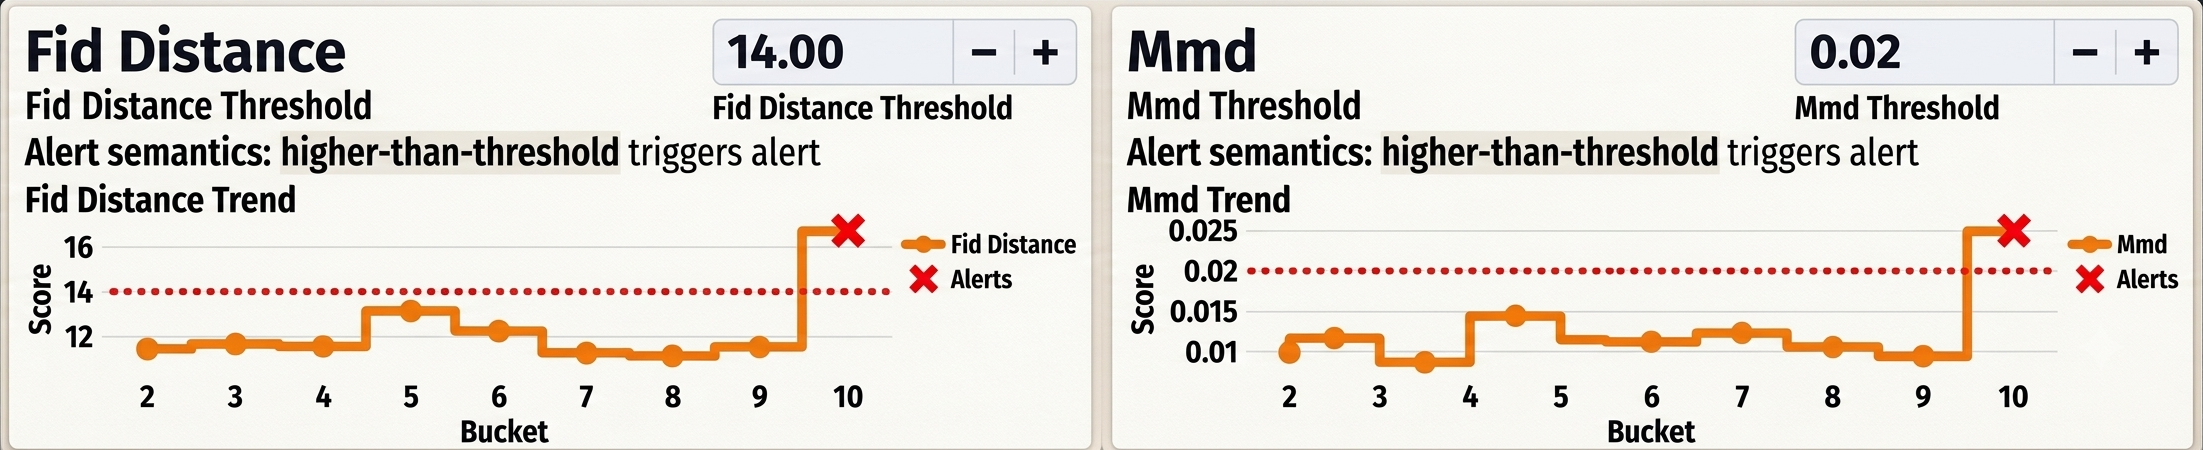
\includegraphics[width=0.90\textwidth]{abcd1.png}

    \vspace{1mm}
    (a)

    \vspace{2mm}

    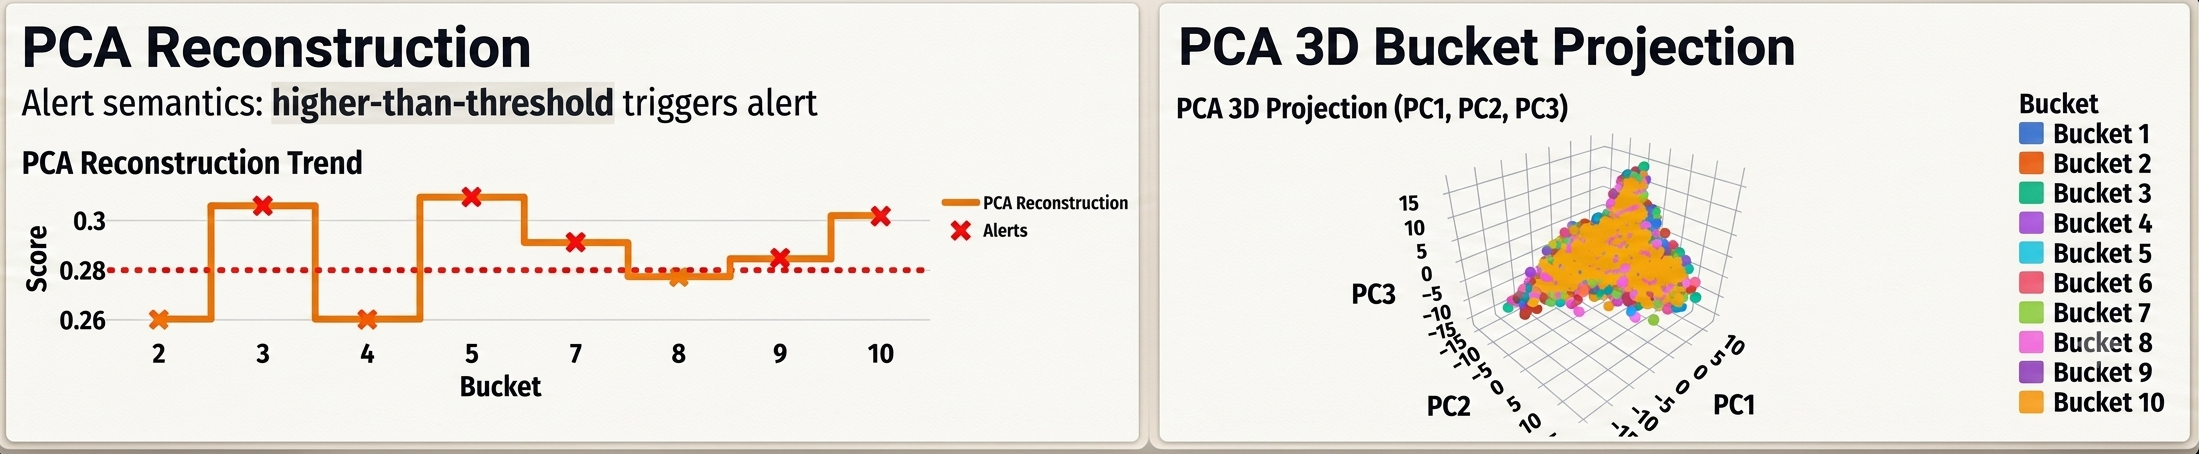
\includegraphics[width=0.90\textwidth]{abcd2.png}

    \vspace{1mm}
    (b)

    \vspace{2mm}

    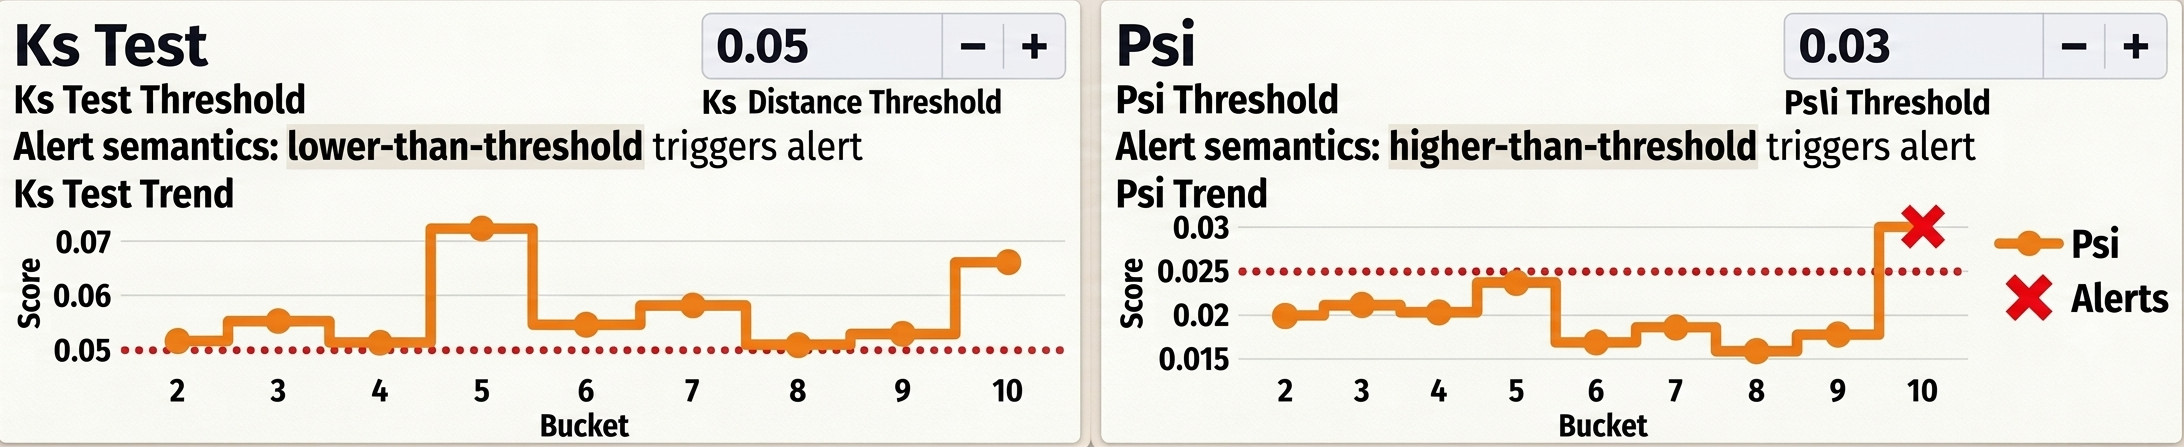
\includegraphics[width=0.90\textwidth]{clear_10-detector.png}

    \vspace{1mm}
    (c)

    \caption{CLEAR-10 multivariate drift analysis: (a) FID and MMD trends; (b) PCA reconstruction trend with a three dimensional bucket projection; (c) detector trends across CLEAR-10 buckets.}
    \label{fig:clear-multivariate}
\end{figure*}

Panels (a) and (b) show the FID, MMD and PCA reconstruction curves staying flat until bucket 10. The projection in panel (b) pulls the later buckets away from bucket 1. Panel (c) places every detector score on one axis, where the KS test leads and the rest follow only at the end.

Localization by class then asks whether the drift in the embeddings is concentrated or spread out. At bucket 10 the background class has 209 of its 512 dimensions at critical severity, while most object classes have only two or three. Root cause analysis ties the largest shifts to error within a class: baseball recall is overestimated by $0.186$ and soccer precision by $0.146$. Fig.~\ref{fig:gradcam} places a few of the worst drifting images next to their Grad-CAM overlays.

\begin{figure*}[!tb]
\centering
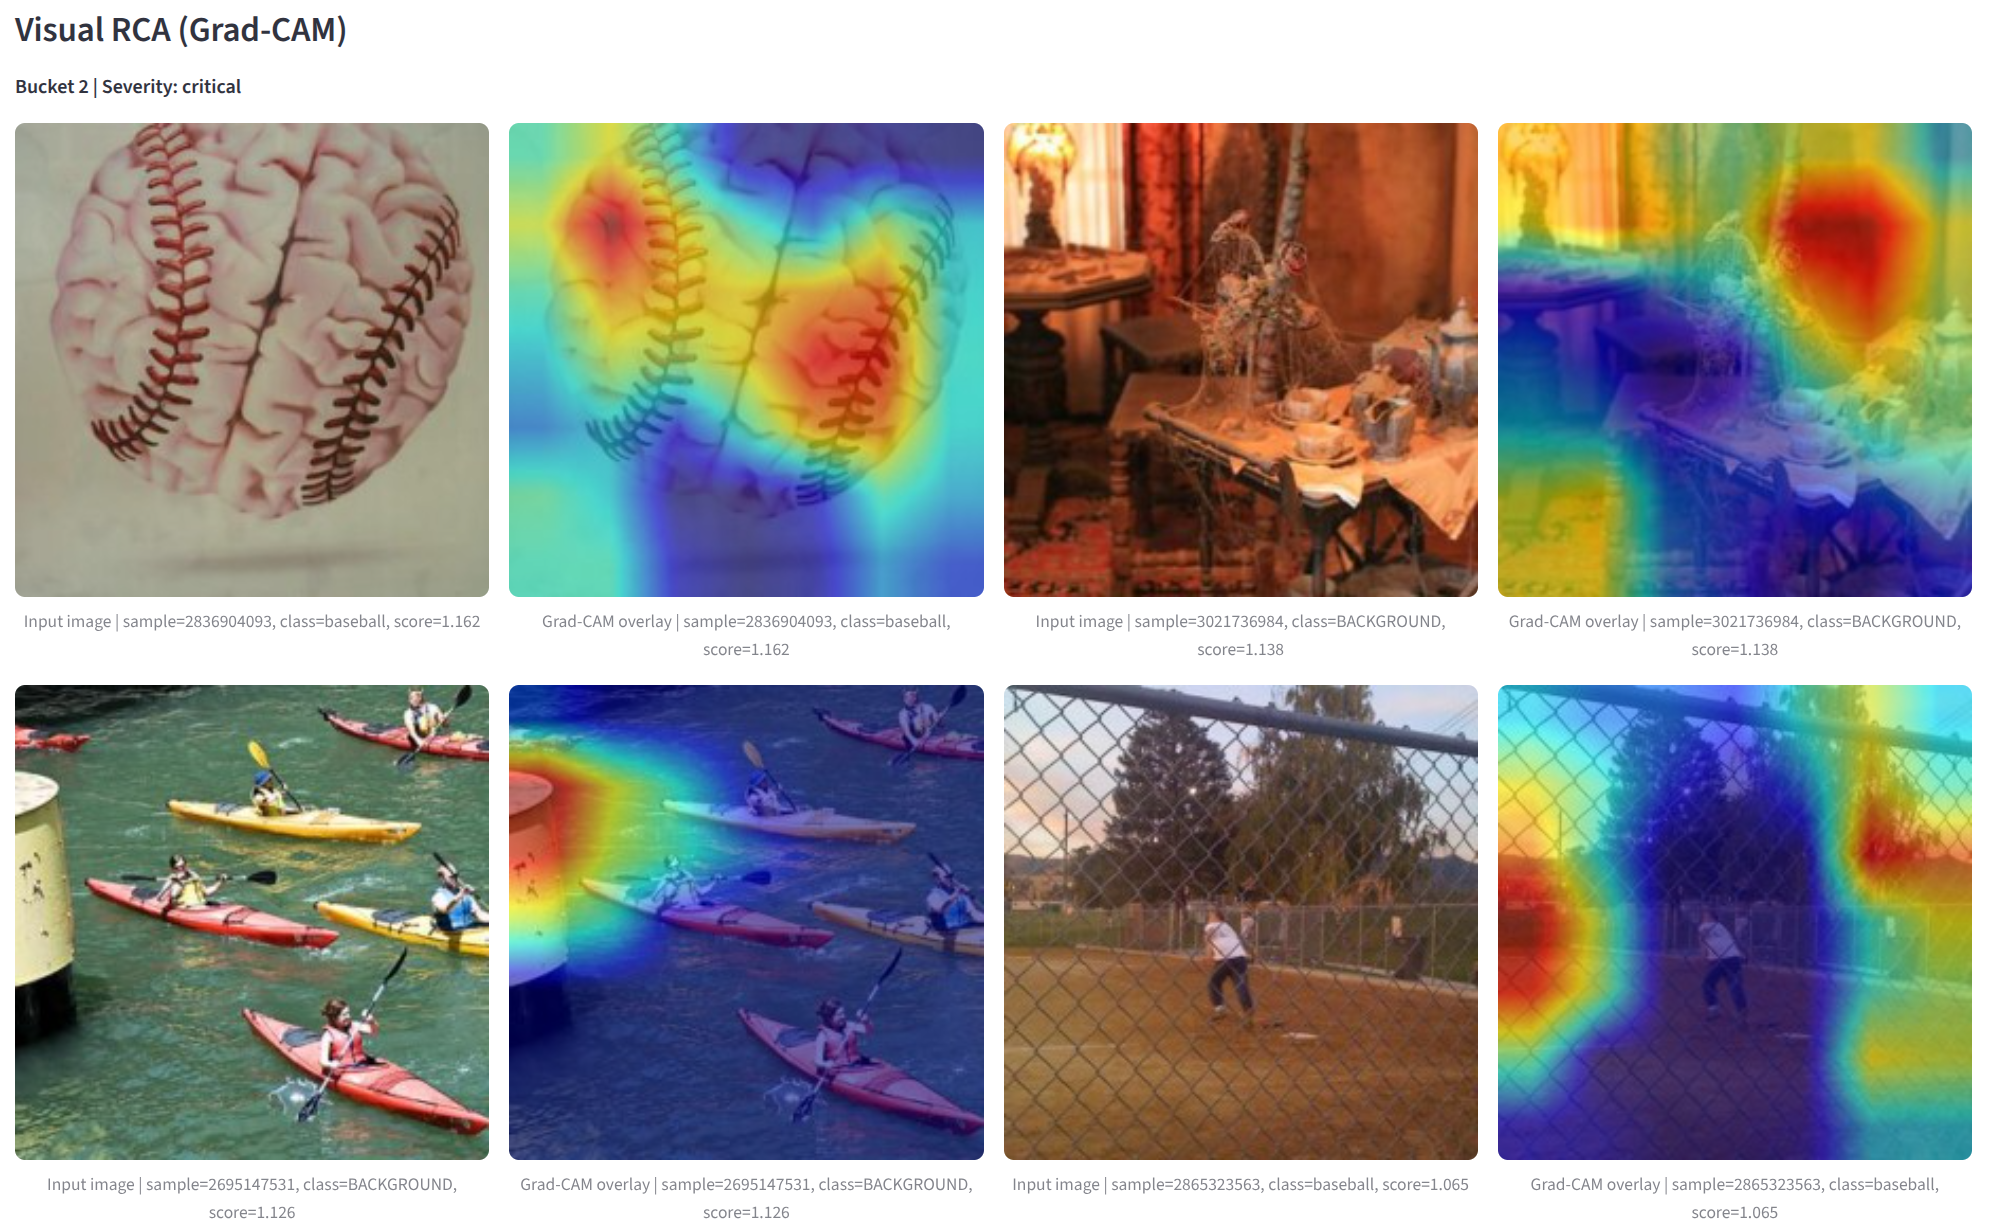
\includegraphics[width=0.90\textwidth,height=0.42\textheight,keepaspectratio]{clear10-gradcam.png}
\caption{CLEAR-10 visual root cause analysis: original images with the matching Grad-CAM overlays.}
\label{fig:gradcam}
\end{figure*}

The overlays show that saliency stays tight on clean objects but scatters in cluttered or dim scenes. This helps separate a change in image content from a change in shooting conditions.

\subsection{Concept level root cause on CLEAR-10}
\label{sec:concept-results}
Section~\ref{sec:architecture} described a concept probe that turns a visual shift into ranked phrases. This subsection checks whether that ranking is right. The test compares the concept mass shift of Equation~(\ref{eq:concept}) against the shift in the image dataset's own automatic tags. Fig.~\ref{fig:concept} shows the ranking for bucket 10, which is the strongest CLEAR-10 shift.

\begin{figure*}[!t]
    \centering
    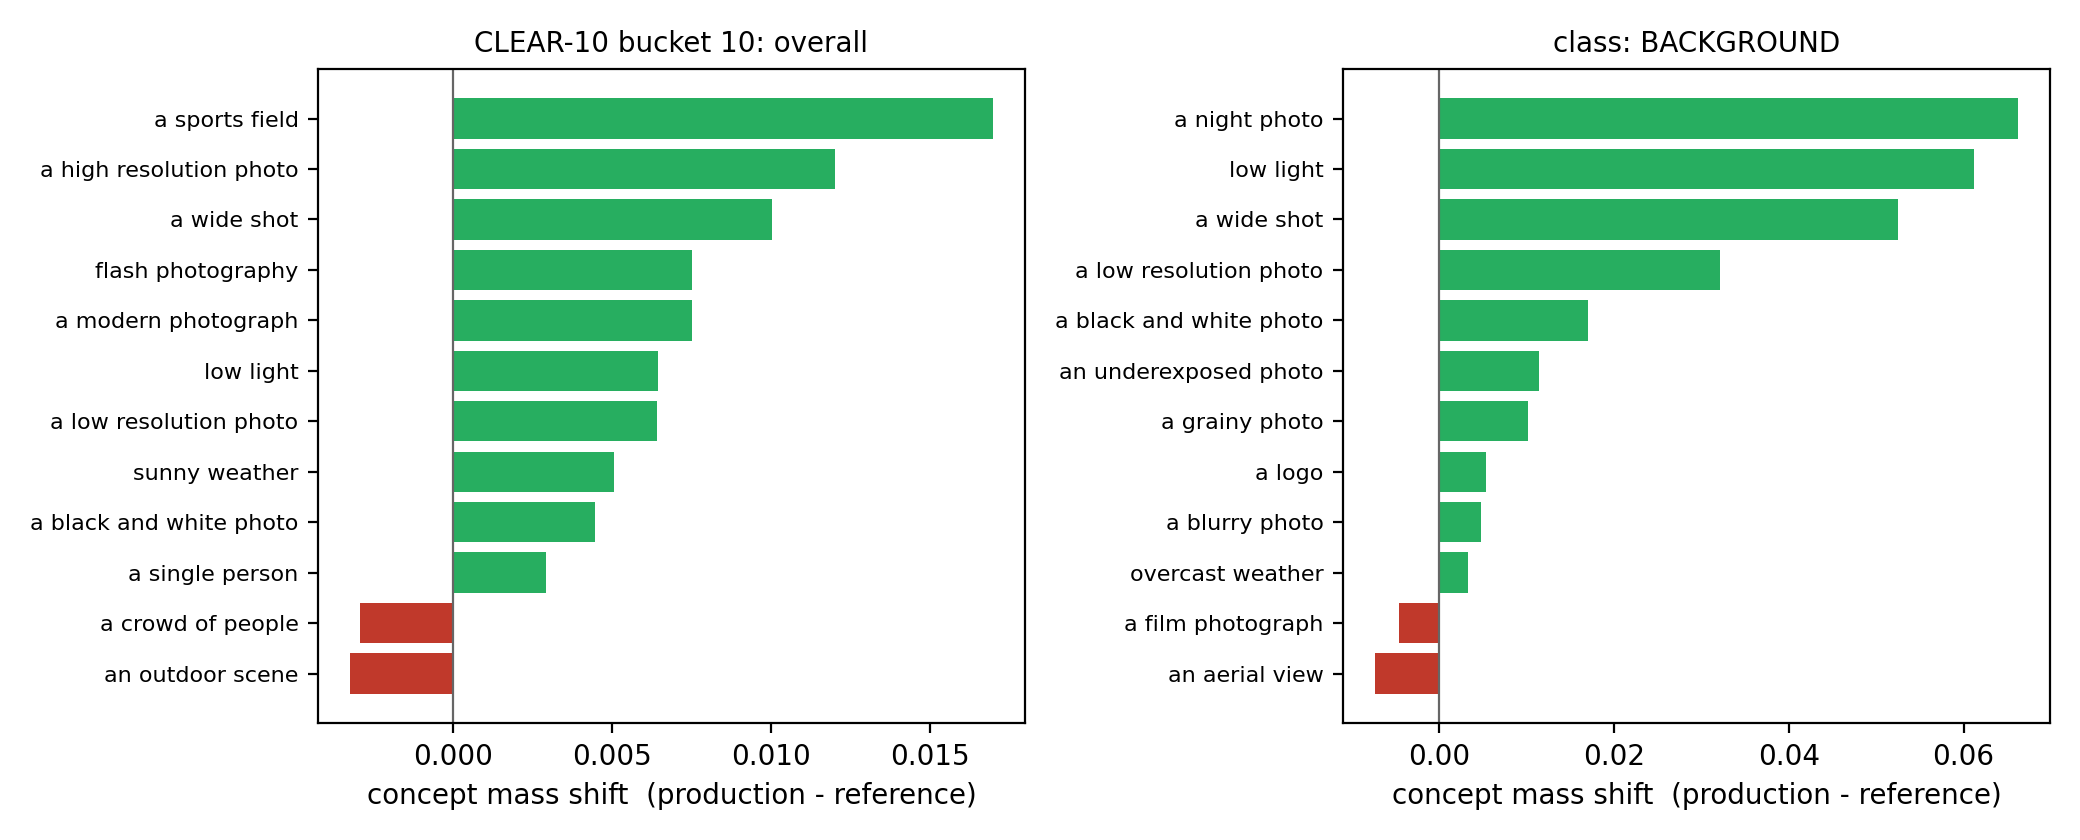
\includegraphics[width=0.92\textwidth]{clip_concept_ranking.png}

    \vspace{1mm}
    (a)

    \vspace{2mm}

    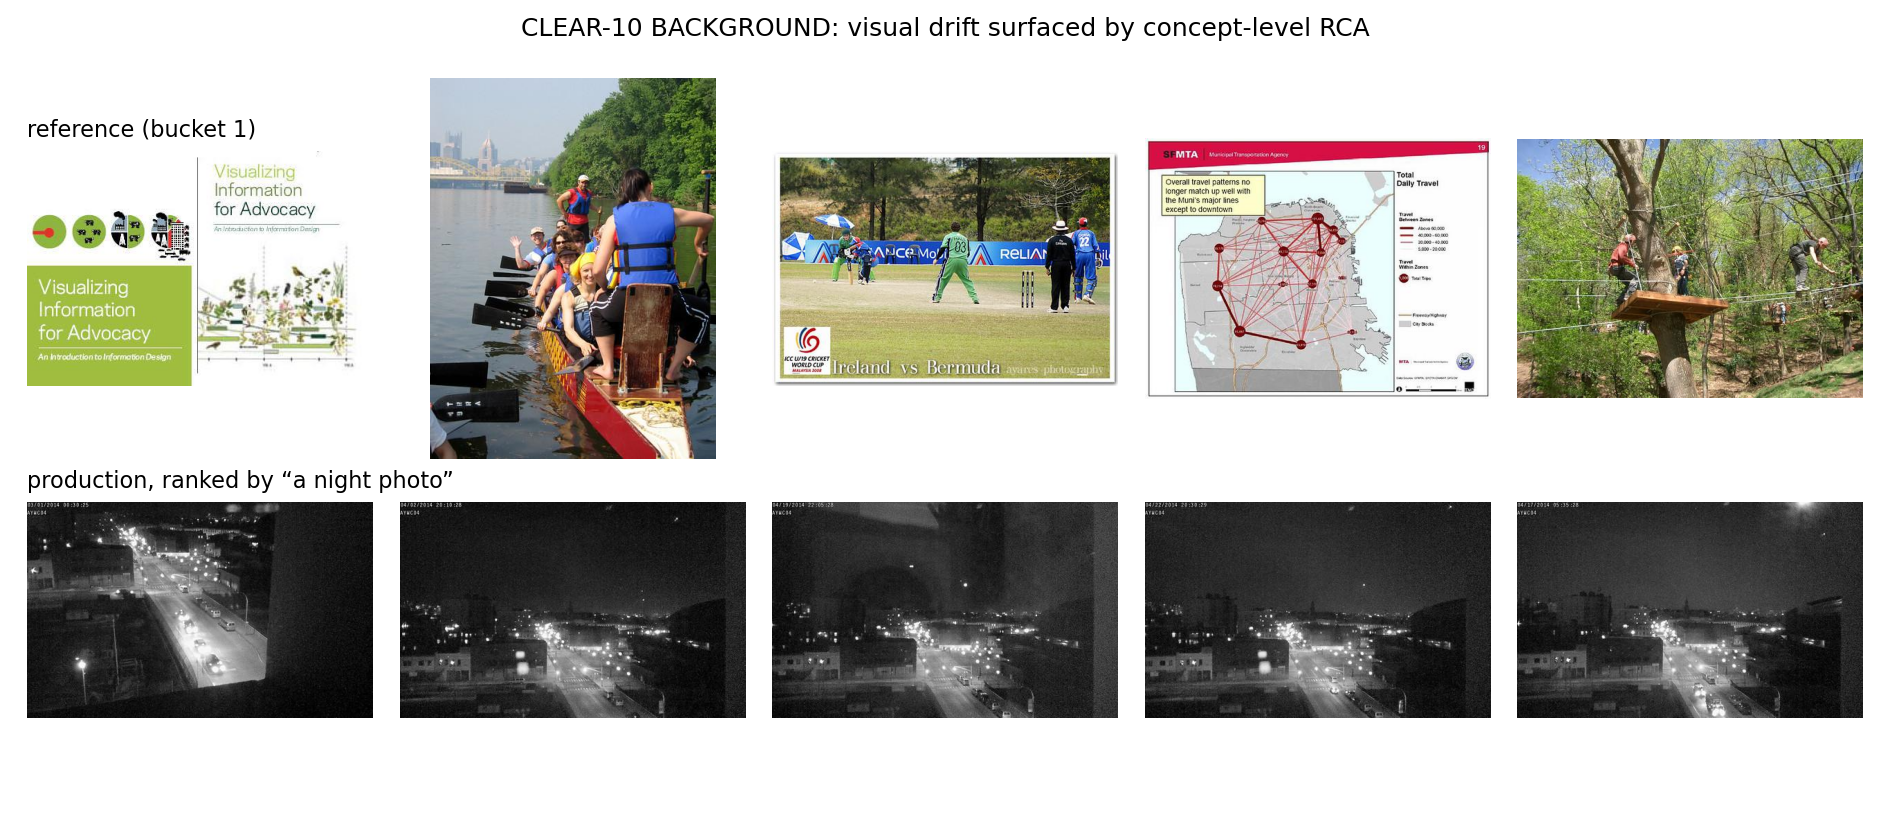
\includegraphics[width=0.80\textwidth]{concept_exemplars.png}

    \vspace{1mm}
    (b)

    \caption{CLEAR-10 bucket 10 concept level root cause: (a) ranked concept mass shift for all classes and for the background class; (b) extreme activation images for the top two drifted embedding dimensions.}
    \label{fig:concept}
\end{figure*}

Fig.~\ref{fig:concept}(a) ranks the phrases whose mass grew most between bucket 1 and bucket 10. For the whole bucket the top gains are a sports field, a wide shot and low light. For the background class the shift is sharper. The phrases night photo, low light, a wide shot, low resolution and black and white all gain mass. Fig.~\ref{fig:concept}(b) shows the images with the most extreme activation on the two top drifting embedding dimensions. The production row is a cluster of night time traffic camera frames, which matches the phrase ranking.

The ranking agrees with the dataset tags. Over the 11 phrases that map to a tag, the Spearman rank correlation between the concept mass shift and the tag shift is $0.71$ ($p = 0.014$). For the background class alone the correlation is again $0.71$ over 8 matched phrases. The median capture year of the background images moves from 2007 in the reference to 2013 in bucket 10, which fits a shift toward newer low light and phone camera imagery. This turns a statement such as ``embedding dimension 342 drifted'' into a cause a data engineer can act on.

\subsection{Proxy estimation quality}
Held out labels are used here for one purpose only, which is measuring how far the estimate misses. Table~\ref{tab:proxy} collects the CLEAR-10 errors over buckets 2 to 10.

\begin{table}[!htbp]
\caption{CLEAR-10 estimation error.}
\label{tab:proxy}
\centering
\renewcommand{\arraystretch}{1.2}
\begin{tabular}{@{}lcc@{}}
\toprule
\textbf{Metric} & \textbf{Mean absolute error} & \textbf{Maximum absolute error} \\
\midrule
Accuracy  & 0.0044 & 0.0105 \\
Recall (macro) & 0.0050 & 0.0114 \\
F1 (macro) & 0.0045 & 0.0098 \\
Precision (macro) & 0.0132 & 0.0235 \\
\bottomrule
\end{tabular}
\end{table}

Table~\ref{tab:proxy} shows that the estimated aggregate accuracy stays within $0.44$ percentage points of the measured value on average, with the worst case at $1.05$ points. Recall and the F1 score miss by about the same margin. Macro precision comes out $1.3$ points too low on average. On ACS Income the same estimator instead reads $0.6$ to $1.6$ points too high as the fixed reference ages, as seen in Table~\ref{tab:acs-temporal}. The aggregate estimate is good enough to gate alerts. The class level numbers are better treated as hints for investigation. Fig.~\ref{fig:clear-proxy} places the estimated and measured accuracy curves side by side.

\begin{figure*}[!tb]
\centering
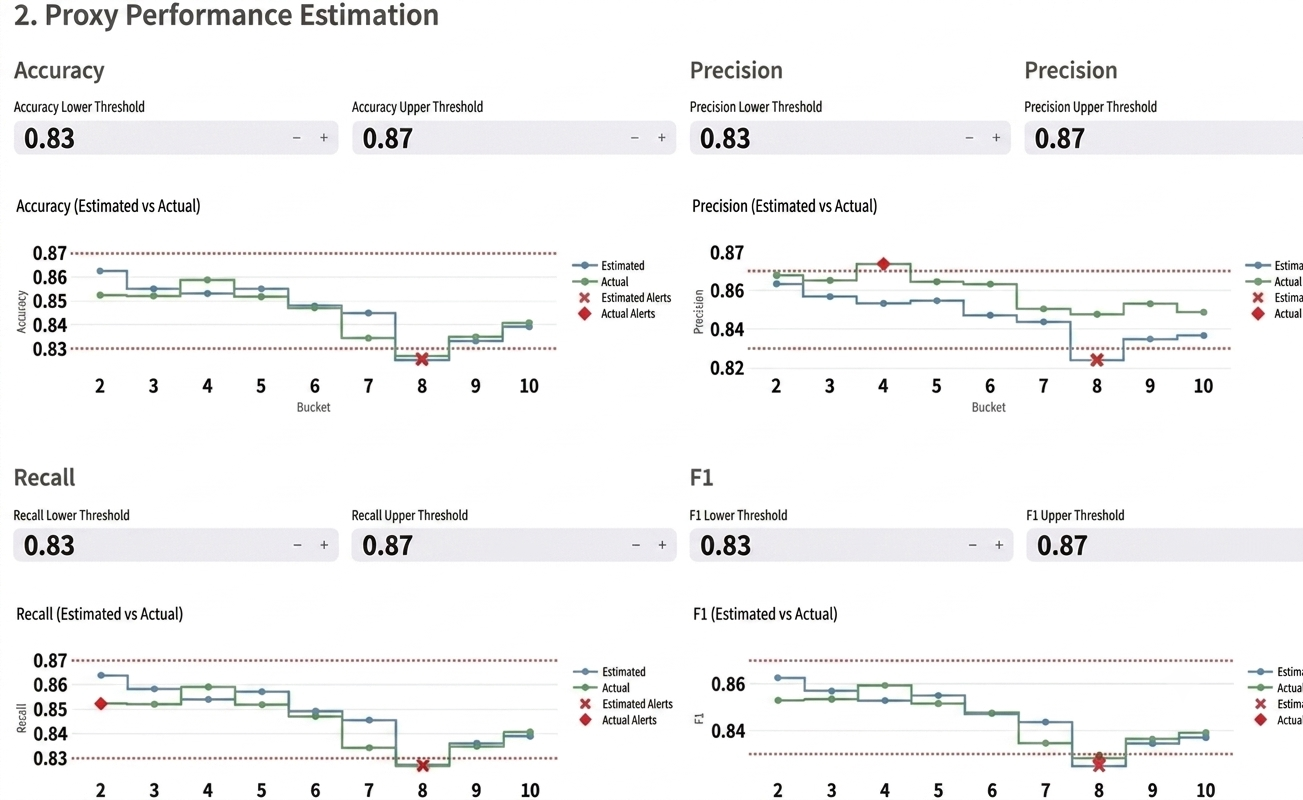
\includegraphics[width=0.90\textwidth]{clear10-proxy.png}
\caption{CLEAR-10 estimated and measured accuracy.}
\label{fig:clear-proxy}
\end{figure*}

The two curves stay close across all nine buckets. The estimate tracks the small dip near bucket 8 and the partial recovery after it.

\subsection{Reliability layer behaviour}
\label{sec:reliability-results}
The reliability analysis asks whether a change in calibration across the population reaches the risk attached to one prediction. Table~\ref{tab:reliability} summarizes the sampled predictions.

\begin{table}[!htbp]
\caption{Prediction reliability scores.}
\label{tab:reliability}
\centering
\renewcommand{\arraystretch}{1.2}
\resizebox{\columnwidth}{!}{%
\begin{tabular}{@{}lcccccc@{}}
\toprule
\textbf{Window} & \textbf{Confidence} & \textbf{OOD risk} & \textbf{Calibration risk} & \textbf{Fused risk} & \textbf{Suspicious} & \textbf{High risk} \\
\midrule
ACS 2015 & 0.793 & 0.06 & 0.231 & 0.104 & 5.5\% & 3.0\% \\
ACS 2016 & 0.794 & 0.05 & 0.238 & 0.101 & 3.0\% & 2.0\% \\
ACS 2017 & 0.797 & 0.07 & 0.239 & 0.107 & 9.5\% & 3.5\% \\
ACS 2018 & 0.804 & 0.09 & 0.256 & 0.114 & 8.0\% & 3.5\% \\
ACS geographic & 0.752 & 0.06 & 0.177 & 0.101 & 4.5\% & 2.0\% \\
CLEAR buckets 2--10 & 0.94--0.97 & 0.03--0.10 & 0.28--0.43 & 0.09--0.12 & 0\% & 1--5\% \\
\bottomrule
\end{tabular}
}
\end{table}

Table~\ref{tab:reliability} averages over 200 predictions for each tabular window and 80 for each image bucket. Calibration risk is the label free overconfidence term from Equation~(\ref{eq:risk}). The suspicious column is the share flagged by the calibration check. The high risk column is the share the override rules push into the top band. The mean fused risk stays in the low band in every window. Two to four percent of individual tabular predictions are still flagged high risk, almost all of them by the rule that fires on a confident prediction over an out of distribution input. On CLEAR-10 confidence sits near $0.96$ while accuracy is near $0.85$, which gives a mean calibration risk near $0.34$. No image window crosses the suspicious threshold. Fused risk stays between $0.09$ and $0.12$.

The tabular rows show why the correction matters. Once the calibration check reads the per bin accuracy estimate instead of a test $p$ value, mean calibration risk rises from $0.231$ in 2015 to $0.256$ in 2018, following the widening gap between confidence and accuracy. A growing minority of predictions crosses the suspicious threshold, reaching $8\%$ by 2018. The geographic run, where the estimate comes closest to the measured value, records the lowest calibration risk and few flags. The signal moves along with the drift instead of saturating.

The mean fused score still hardly budges. The OOD term is small. A single later census record looks close to an ordinary row, so its out of distribution score sits between $0.05$ and $0.09$, though it does climb as the drift grows. Stability under perturbation stays near zero because the output of a linear model changes smoothly when small noise is added. Equation~(\ref{eq:risk}) then averages a calibration term near $0.25$ against small point level terms and a confidence term near $0.20$, which lands near $0.10$ and inside the low band. In every window the population signal is outvoted by the point level ones. Section~\ref{sec:benchmark-results} measures this weakness against a known ground truth.

\subsection{Remediation triage}
\label{sec:remediation-results}
The triage of Section~\ref{sec:architecture} claims to predict whether retraining will help. This subsection tests that claim on five settings: the ACS temporal shift, the ACS geographic shift to Washington, one controlled covariate shift on ACS and CLEAR-10 buckets 6 and 10. Table~\ref{tab:triage} reports the outcome.

\begin{table}[!htbp]
\centering
\caption{Remediation triage across five drift settings.}
\label{tab:triage}
\renewcommand{\arraystretch}{1.2}\setlength{\tabcolsep}{3pt}\scriptsize
\begin{tabular}{@{}l r l r r r l@{}}
\toprule
setting & gap (pp) & cheapest fix & recovered & cost (s) & full retrain & triage \\
\midrule
ACS temporal & 1.8 & retrain on recent & 12\% & 0.10 & 11\% & do not retrain \\
ACS geographic & 2.3 & importance weighted & 5\% & 0.04 & 0\% & do not retrain \\
ACS synthetic covariate shift & 7.7 & feature drop & 56\% & 0.02 & 0\% & escalate \\
CLEAR-10 bucket 6 & 2.5 & retrain on recent & 41\% & 0.75 & 99\% & escalate \\
CLEAR-10 bucket 10 & 3.2 & retrain on recent & 92\% & 0.69 & 82\% & escalate \\
\bottomrule
\end{tabular}
\end{table}

Table~\ref{tab:triage} lists, for each setting, the accuracy gap, the recovery of the cheapest label free probe, the recovery of a full retrain and the triage verdict. On the two real ACS shifts no strategy recovers more than $0.2$ points. Dropping the KS localized features is worse than doing nothing, since those features carry the decision. Accuracy falls by 18 points on the temporal shift and 14 points on the geographic shift when they are removed. The triage reads the weak probe recovery and advises against a retrain. On the controlled covariate shift, where the cause is a known rescaling of two features, importance weighting recovers 55 percent of the gap with no labels and the triage escalates. On CLEAR-10 retraining on the previous bucket recovers 41 percent of the gap for bucket 6 and 92 percent for bucket 10, each in under a second, against a full retrain that costs 4 to 12 seconds. The triage escalates in both cases. Fig.~\ref{fig:remediation-pareto} places recovery against fitting cost for these settings.

\begin{figure}[!htbp]
\centering
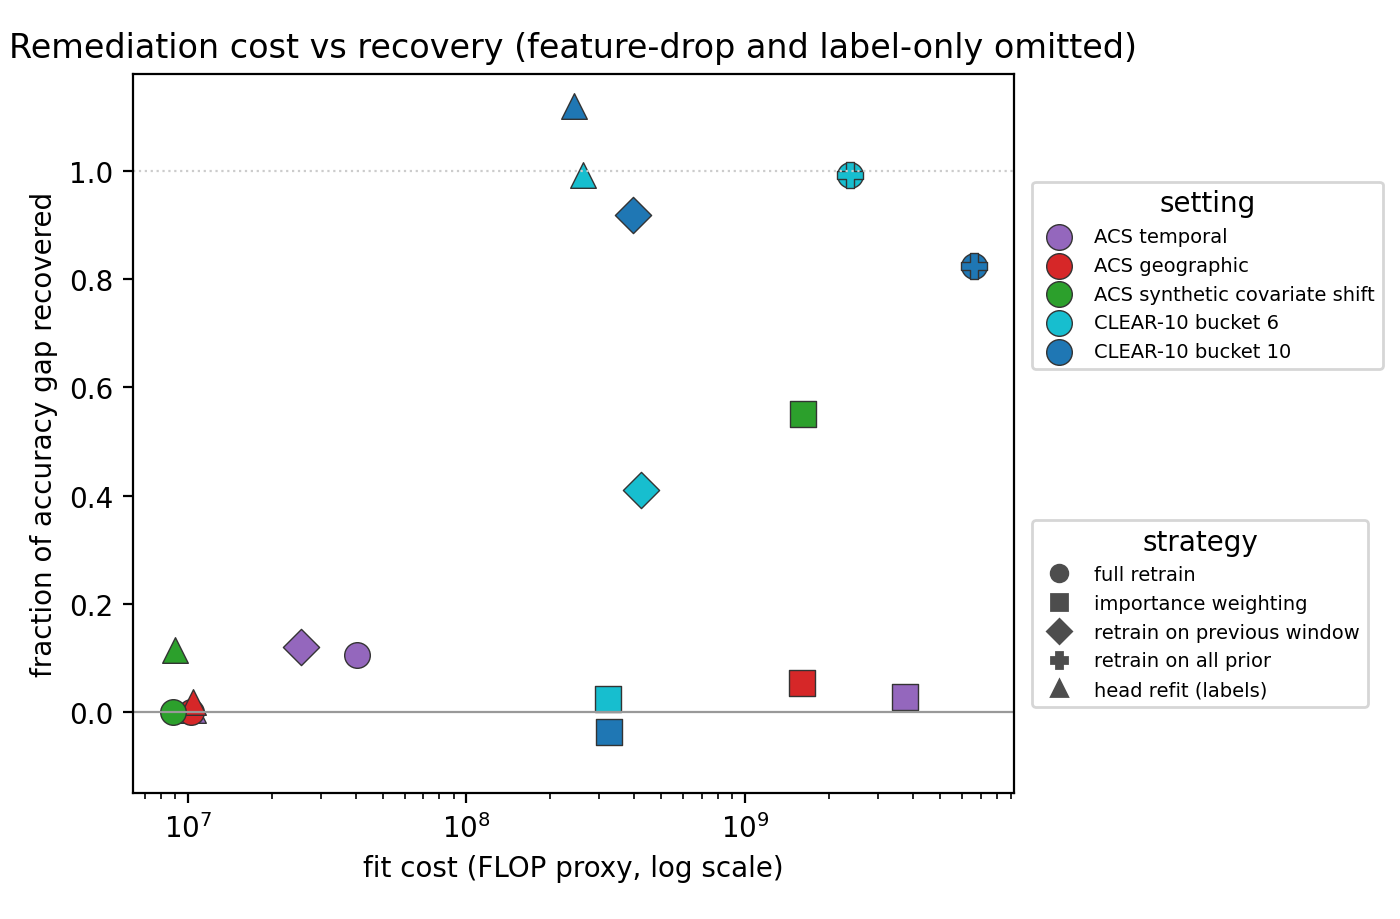
\includegraphics[width=0.95\columnwidth]{remediation_pareto.png}
\caption{Remediation recovery against fitting cost across five settings.}
\label{fig:remediation-pareto}
\end{figure}

Fig.~\ref{fig:remediation-pareto} shows that the cheap strategies sit on the cost against recovery frontier for the recoverable shifts, while every strategy sits near zero recovery for the real ACS shifts. The verdict was correct for all five settings. The lesson is that separability is not the same as recoverability. The geographic shift is highly separable, with a domain classifier area under the curve of $0.85$, yet none of its accuracy loss can be recovered by retraining on the old target rule.

\subsection{Drift injection benchmark}
\label{sec:benchmark-results}
The benchmark of Section~\ref{sec:benchmark-setup} grades every stage of the pipeline against a known ground truth. Table~\ref{tab:injection-benchmark} reports the strongest intensity of each drift type.

\begin{table}[!htbp]
\centering
\caption{Drift injection benchmark results at the strongest injected intensity.}
\label{tab:injection-benchmark}
\renewcommand{\arraystretch}{1.25}\setlength{\tabcolsep}{3pt}\scriptsize
\begin{tabular}{@{}l r r r c c l l@{}}
\toprule
injected & true drop & label-free & audit & KS loc.\ & rel.\ & type & remediation \\
 & (pp) & err.\ (pp) & err.\ (pp) & F1 & AUROC & verdict & verdict \\
\midrule
no drift & -1.1 & -1.1 & -1.1 & clean & -- & none & -- \\
covariate & +16.4 & +23.2 & +3.1 & 1.00 & 0.56 & covariate & escalate (ok) \\
prior & +4.3 & +1.6 & +0.7 & -- & 0.47 & prior & hold (ok) \\
concept & +24.8 & +24.8 & +0.3 & 0.00 & 0.43 & concept & hold (ok) \\
label noise & +18.9 & +18.9 & -1.3 & clean & 0.51 & label noise & hold (ok) \\
\bottomrule
\end{tabular}
\end{table}

Table~\ref{tab:injection-benchmark} shows that the pipeline names the injected drift type in all 13 windows, including the no drift control. Covariate and prior shift are resolved from label free signals. Concept drift and label noise leave the inputs and the model outputs unchanged, so no label free monitor can see them. The pipeline reports this. The 600 label audit then resolves the type. The label free accuracy estimate is optimistic in every window. Under covariate shift it rises as true accuracy falls, reaching an error of 23 points, because the rescaled features make the model more confident. Under concept drift and label noise the estimate does not move at all, so its error equals the full accuracy drop, up to 25 points. The 600 label audit brings the estimate back to within 3 points in every case.

Fig.~\ref{fig:injection} shows how the drift types are told apart and how the pipeline responds to intensity.

\begin{figure*}[!t]
    \centering
    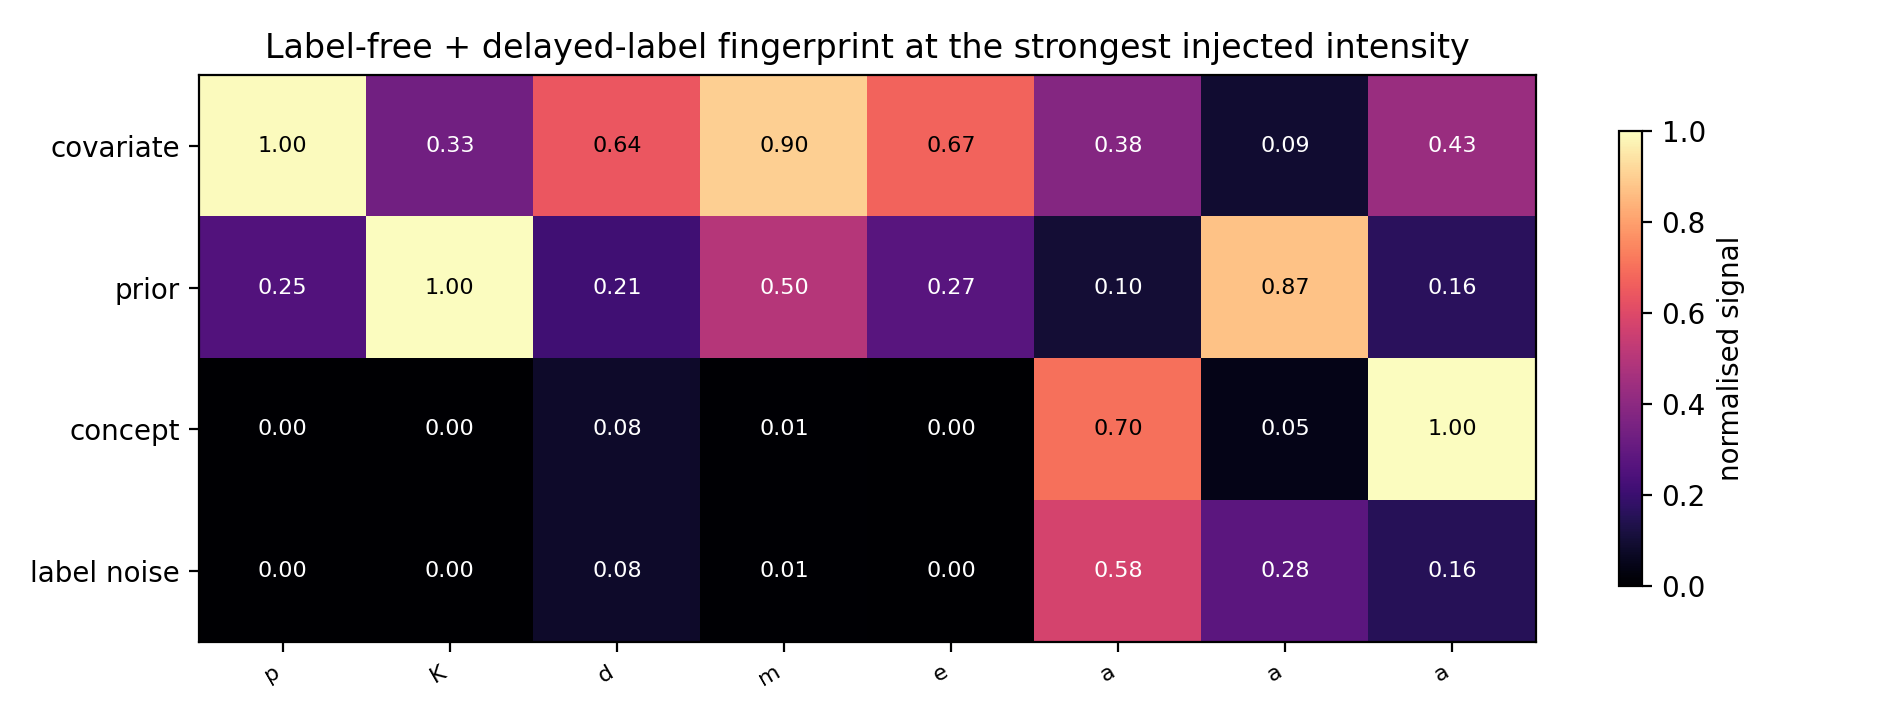
\includegraphics[width=0.88\textwidth]{injection_signature.png}

    \vspace{1mm}
    (a)

    \vspace{2mm}

    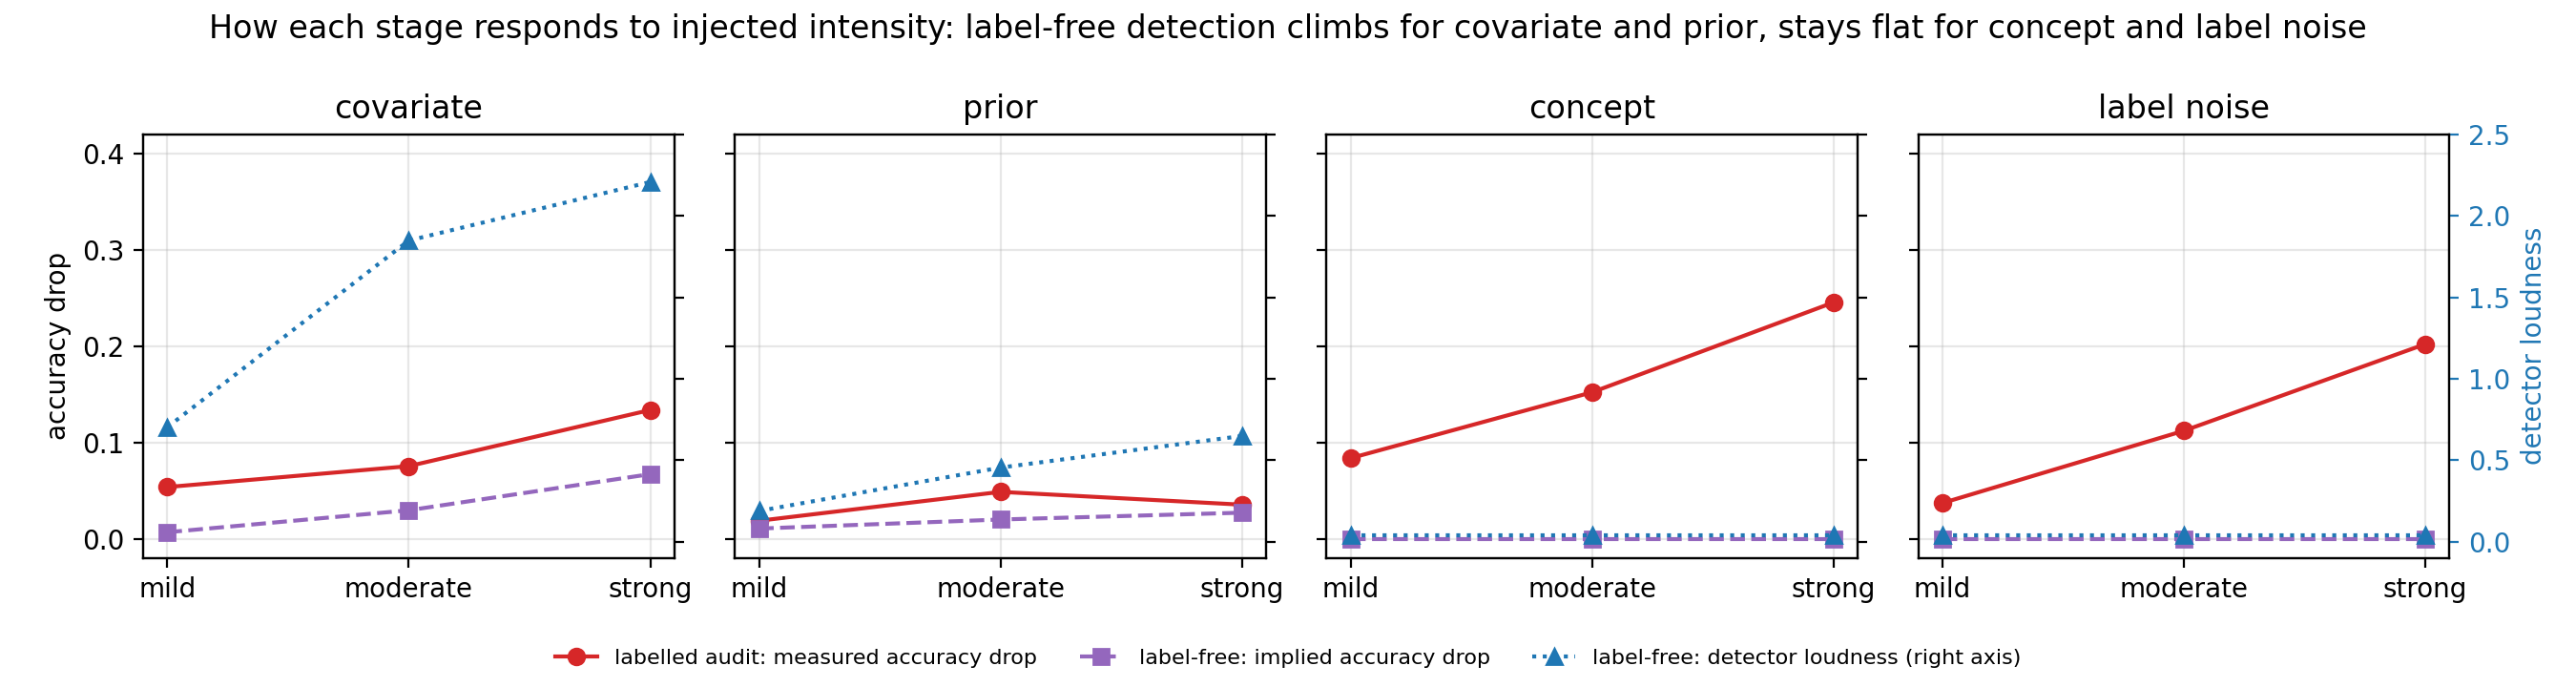
\includegraphics[width=0.95\textwidth]{injection_intensity_response.png}

    \vspace{1mm}
    (b)

    \caption{Drift injection benchmark: (a) label free and delayed label fingerprint at the strongest intensity; (b) response of each stage to injected intensity.}
    \label{fig:injection}
\end{figure*}

Fig.~\ref{fig:injection}(a) is the label free and audit fingerprint at the strongest intensity. Covariate shift lights up the input detectors and the domain separability. Prior shift moves the model's own positive rate. Concept drift and label noise leave every label free signal near zero and are separated only by the audit, which finds the loss concentrated in the education range for concept drift and spread evenly for label noise. Fig.~\ref{fig:injection}(b) shows that label free detector strength climbs with intensity for covariate and prior shift but stays flat for concept drift and label noise. The audit's measured drop climbs for all four. Localization matches the injected features for covariate shift, with an F1 score of $1.0$. The audit names the concept region feature every time.

The reliability score is informative only for covariate shift, where its AUROC against prediction error is $0.56$. For concept drift the AUROC is $0.43$, below chance, because the model is confidently wrong exactly where the rule changed. For label noise it is $0.51$, since the predictions are not wrong. The labels are. This is the same limitation seen on the real ACS stream in Section~\ref{sec:reliability-results}. The benchmark shows why. The triage escalates a retrain only for covariate shift, which matches the fix each drift needs.

\subsection{Runtime}
On the 2018 ACS window, which holds about 196{,}000 rows and 10 features, one detector pass with localization runs in $0.5$ to $1.6$ seconds. The KS pipeline with Shapley analysis on 200 samples takes $1.6$ seconds. MMD with 20 permutations on a 3{,}000 row subsample takes $5.9$ seconds. The cost of reliability is dominated by the five perturbed predictions made for every sampled record. For CLEAR-10 the biggest one time cost is pulling embeddings out of roughly 33{,}000 images. The concept probe adds one CLIP pass over the sampled images. The injection benchmark runs the whole pipeline on 13 windows in a few minutes on the same workstation.

\section{Comparative Study with Related Work}
\label{sec:comparative}

This comparison sets the proposed pipeline next to three representative research methods. Rabanser et al. study statistical tests for spotting dataset shift \cite{rabanser2019failing}. Kivim\"aki et al. estimate classification performance from confidence when no production labels exist \cite{kivimaki2025performance}. Ovadia et al. examine predictive uncertainty and calibration under dataset shift \cite{ovadia2019trust}. Concept level explanation is closest to Testing with Concept Activation Vectors \cite{kim2018tcav}, which needs gradients and a trained probe, while the probe here needs neither. Table~\ref{tab:comparative} lines up what each method covers against the integrated pipeline.

\begin{table}[!htbp]
\centering
\caption{Comparison with related methods.}
\label{tab:comparative}
\renewcommand{\arraystretch}{1.25}
\setlength{\tabcolsep}{2.5pt}
\scriptsize
\begin{tabular}{|>{\raggedright\arraybackslash}m{2.35cm}|>{\centering\arraybackslash}m{1.1cm}|>{\centering\arraybackslash}m{1.0cm}|>{\centering\arraybackslash}m{1.0cm}|>{\centering\arraybackslash}m{1.1cm}|}
\hline
\multicolumn{1}{|c|}{\textbf{Capability}} &
\textbf{\shortstack{Rabanser\\et al.}} &
\textbf{\shortstack{Kivim\"aki\\et al.}} &
\textbf{\shortstack{Ovadia\\et al.}} &
\textbf{Proposed} \\
\hline
Drift detection & $\checkmark$ & -- & -- & $\boldsymbol{\checkmark}$ \\
\hline
Performance estimation & -- & $\checkmark$ & -- & $\boldsymbol{\checkmark}$ \\
\hline
Drift localization & Limited & -- & -- & $\boldsymbol{\checkmark}$ \\
\hline
Root cause analysis & -- & -- & -- & $\boldsymbol{\checkmark}$ \\
\hline
Concept level explanation & -- & -- & -- & $\boldsymbol{\checkmark}$ \\
\hline
Calibration analysis & -- & Limited & $\checkmark$ & $\boldsymbol{\checkmark}$ \\
\hline
Prediction level reliability & -- & -- & $\checkmark$ & $\boldsymbol{\checkmark}$ \\
\hline
Remediation with cost analysis & -- & -- & -- & $\boldsymbol{\checkmark}$ \\
\hline
Controlled drift type evaluation & -- & -- & -- & $\boldsymbol{\checkmark}$ \\
\hline
Integrated diagnosis & -- & -- & -- & $\boldsymbol{\checkmark}$ \\
\hline
\end{tabular}
\end{table}

Table~\ref{tab:comparative} mirrors the main aim of each study. Rabanser et al. contribute sensitive tests for shift with a limited view at the sample level. Kivim\"aki et al. estimate aggregate performance from calibrated confidence. Ovadia et al. judge the quality of uncertainty under shift. The proposed pipeline draws these aims into one workflow. It adds localization at the level of a feature or a slice, root cause analysis based on SHAP, Grad-CAM and a concept probe, per prediction reliability scoring, a remediation triage and a benchmark that grades each stage against a known drift type.

\section{Limitations}
\label{sec:limits}

The limitations mark where the reported evidence should not be stretched. The main one is in reliability fusion. A calibration signal measured over a population is averaged with smaller point level signals, so it rarely lifts the mean risk label. The benchmark puts a number on this. The reliability score separates errors only under covariate shift, with an AUROC of $0.56$. It drops below chance under concept drift.

Label free monitors cannot see concept drift or label noise when the inputs and the model outputs do not change. This is a property of the setting, not a bug. The delayed label audit needs a few hundred labels to resolve these cases.

The concept vocabulary is a fixed list of English phrases. CLIP carries the bias of its own training data. The automatic tags used for validation are noisy. The concept result is clean for the strongest CLEAR-10 shift and weaker for the milder ones.

Static thresholds can overreact to changes that are significant but small in practice. The accuracy estimate is built on a fixed reference and goes stale, reading up to $1.6$ points too high on ACS as the reference ages. The pipeline runs in batches. It advises but does not retrain, roll back or talk to a scheduler.

Only two datasets, two modalities and linear decision rules were tested. The benchmark injects one drift type at a time, while real drift is often a mix of several.

\section{Conclusion and Future Work}

The study shows that signals which need no labels can hold together a single monitoring workflow across tabular and image models. The pipeline goes from a label free accuracy estimate to a named cause and a remediation verdict.

On real drift the pipeline followed a gradual two point loss on ACS Income and named the features whose influence was changing. On CLEAR-10 it produced a ladder of detector sensitivity along with accurate aggregate estimates. The concept probe turned image drift into readable causes that agree with the dataset tags at a rank correlation of $0.71$. The remediation triage predicted, for every tested setting, whether retraining would recover the loss.

The injection benchmark tied the evidence together. The pipeline named every injected drift type. The label free accuracy estimate was optimistic in every window. For concept drift and label noise it did not move at all. Per prediction reliability helped only under covariate shift. The benchmark also confirmed the fusion weakness in the reliability layer.

The immediate plan is to let a sustained population level signal raise the risk label on its own, as the current rules already do for a high OOD score. A second plan is to tie thresholds to the estimated loss in performance. Later work includes streaming execution, tests on mixed drift, a learned concept vocabulary and support for text.

\bibliographystyle{IEEEtran}
\bibliography{references}

\end{document}
